\documentclass[a4paper, 11pt]{article}
%\documentclass[english,m,master,binding,twoside,palatino,nogermanabstract]{thesis}
\usepackage{a4wide}
\usepackage[english]{babel}
\usepackage[T1]{fontenc}
\usepackage[utf8]{inputenc}
\usepackage{times}
\usepackage{ifthen}
\usepackage{here}

\usepackage[style=apa, backend=biber]{biblatex}
\DeclareLanguageMapping{english}{american-apa}
\addbibresource{bib.bib}

\usepackage{graphicx}
\graphicspath{{./images/}}
\DeclareGraphicsExtensions{.pdf,.jpeg,.png,.svg}
\usepackage{hyperref}
\usepackage{movie15}
\usepackage{fixltx2e}
\usepackage{amsmath}
\usepackage{amssymb}
\usepackage{nccmath}
\usepackage{csquotes}
\usepackage{multirow}
\usepackage{array}
\usepackage{booktabs}
\usepackage{listings}
\usepackage{float}
\usepackage{color}
\usepackage{graphicx}
\usepackage{blindtext}
\usepackage{color}

% ---------------------------------------------
%	Commands definition
% ---------------------------------------------
\newcommand{\R}{\mathbb{R}}
\newcommand{\myName}{Kandhasamy Rajasekaran}
\newcommand{\emailID}{kandhasamy@uni-koblenz.de}
\newcommand{\matriculationID}{216100855}
\newcommand{\Title}{Deep Learning techniques applied to Constituency parsing of German}
\newcommand{\supervisor}{Prof. Dr. Karin Harbusch} %inkl. Titel
\newcommand{\secondSupervisor}{Denis Memmesheimer} %inkl. Titel

\topmargin 0cm \textheight 23cm \parindent 0cm
\setlength{\parindent}{2em}


\begin{document}

\thispagestyle{empty}

%%%%%%%%%%%%%%%%%%%%%%%%%%%%%%%%%%%%%% Title page %%%%%%%%%%%%%%%%%%%%%%%%%%%%%%%%%%%%%%%%%%%

\begin{titlepage}
\enlargethispage{3em}

\begin{minipage}{0.45\textwidth}
  \begin{flushleft} \small
    
\includegraphics[width=68mm]{Uni-Logo}
    \hspace*{16mm}Fachbereich 4: Informatik
  \end{flushleft}
\end{minipage}
\hfill
\begin{minipage}{0.45\textwidth}
  \begin{flushright} \small
  %
\includegraphics[bb=0 -120 706 298,height=40mm]{cvlogo.png} \\
   
\includegraphics[width=40mm, height=10mm]{cvlogo.png}
     {\ }
  \end{flushright}
\end{minipage}

\hspace*{10mm}
\begin{minipage}[b]{0.8\textwidth}
  \begin{flushleft}
  \vspace{2cm}  
 
\begin{center}

\Huge{\bf \Title} \\
\vspace{4em}

%%% UNTERTITEL
\LARGE{
	Master's Thesis
} % end of \Large

\hspace*{10mm}
\normalsize{
	in partial fulfillment of the requirements for the degree of \\
	 Master of Science (M.Sc.) in Web Science
}
\vspace{2em}

\small{Submitted by} \\
\Large{
  \myName
}
\vspace{6em}

\end{center}

  \footnotesize{
      {\bf Betreuer:} 
	  	\supervisor{}, Institut für Computervisualistik, Fachbereich Informatik, Universität Koblenz-Landau \\
      {\bf Erstgutachter:}   % Formal vorgegeben: immer DP
	  	\supervisor{}, Institut für Computervisualistik, Fachbereich Informatik, Universität Koblenz-Landau \\
      {\bf Zweitgutachter:}  % Gutachter muss mindestens den akademischen Grad der Arbeit haben
	  	\secondSupervisor{}, Institut für Computervisualistik, Fachbereich Informatik, Universität Koblenz-Landau \\
    % hier Abgabemonat und -jahr eintragen
    
    \vspace{1em}
    \begin{flushleft}
    Koblenz, im Januar 2020
    \end{flushleft}
 }

%First supervisor:\hspace{2mm} \supervisor{}, Institute for Computer Visualistics \\
%Second supervisor:\hspace{2mm} \secondSupervisor{}, Institute for Computer Visualistics \\

\end{flushleft}
\end{minipage}

\end{titlepage}
\pagebreak

%%%%%%%%%%%%%%%%%%%%%%%%%%%%%%%%%%%%%% Statements %%%%%%%%%%%%%%%%%%%%%%%%%%%%%%%%%%%%%%%%%%%
        \begin{flushleft}
            \begin{Large}
                Statement
              \\[5mm]
            \end{Large}
              I hereby certify that this thesis has been composed by me and is based on my own work, that I did not use any further resources than specified \textendash{} in particular no references unmentioned in the reference section \textendash{} and that I did not submit this thesis to another examination before. The paper submission is identical to the submitted electronic version.
            \\[.75cm]
            \begin{center}
            \begin{tabular}{l p{1cm} cc}
              \empty & \empty & 
                Yes
              & 
                No
              \\[.5cm]
                I agree to have this thesis published in the library.& \empty & $\square$ & $\square$\\[.5cm]
                I agree to have this thesis published on the Web.& \empty & $\square$ & $\square$\\[.5cm]
                The thesis text is available under a Creative Commons  & \empty & \empty & \empty\\
                License (CC BY-SA 4.0). & \empty & $\square$ & $\square$\\[.5cm]
                The source code is available under a GNU General Public & \empty & \empty & \empty\\
                License (GPLv3). & \empty & $\square$ & $\square$\\[.5cm]
                The collected data is available under a Creative Commons & \empty & \empty & \empty\\
                License (CC BY-SA 4.0). & \empty & $\square$ & $\square$\\[.5cm]
            \end{tabular}\\[2cm]
            \end{center}
            \begin{small}
              \dotfill\\
                (Place, Date)\hfill(Signature)
            \end{small}
            \cleardoublepage%
          %\repeat%
        \end{flushleft}
\pagebreak

%%%%%%%%%%%%%%%%%%%%%%%%%%%%%%%%%%%%%% Note %%%%%%%%%%%%%%%%%%%%%%%%%%%%%%%%%%%%%%%%%%%

\vspace{2em}
        \begin{flushleft}
        	\begin{Large}
                	Note
              \\[5mm]
        	\end{Large}
            \begin{itemize}
            	\item If you would like us to contact you for the graduation ceremony, 
                \item[] please provide your personal E-mail address: \dotfill
                \item If you would like us to send you an invite to join the WeST Alumni 
                \item[] and Members group on LinkedIn, please provide your LinkedIn ID : \dotfill
            \end{itemize}
            \cleardoublepage%
        \end{flushleft}
\pagebreak      

%%%%%%%%%%%%%%%%%%%%%%%%%%%%%%% Acknowledgements %%%%%%%%%%%%%%%%%%%%%%%%%%%%%%%%%%%%%%%%%%%%


\vspace*{\fill}
I would like to express my gratitude to my advisors Prof.Dr.Karin Harbusch and Denis Memmesheimer for their support throughout the course of my Master thesis. Thank you.

My mother has been very supportive of me and all those weekly phone calls have helped me to put things in perspective. Thank you.
\vspace*{\fill}


    \selectlanguage{english}
  \cleardoublepage%  
\pagebreak        

%%%%%%%%%%%%%%%%%%%%%%%%%%%%%%%%%%%%%% Abstract %%%%%%%%%%%%%%%%%%%%%%%%%%%%%%%%%%%%%%%%%%%

\begin{abstract}

Constituent parsing attempts to extract syntactic structure from a sentence. These parsing systems are helpful in many NLP applications such as grammar checking, question answering, and information extraction. This thesis work is about implementing a constituent parser for German language using neural networks. Over the past, recurrent neural networks have been used in building a parser and also many NLP applications. In this, self-attention neural network modules are used intensively to understand sentences effectively. With multi-layered self-attention networks, constituent parsing achieves 93.68\% F1 score. This is improved even further by using both character and word embeddings as a representation of the input. An F1 score of 94.10\% was the best achieved by constituent parser using only the dataset provided. With the help of external datasets such as German Wikipedia, pre-trained ELMo models are used along with self-attention networks achieving 95.87\% F1 score.
\end{abstract}
\vspace*{5em}  
\begin{center}
\textbf{Zusammenfassung} \\
\end{center}
Konstituenten-Parsing versucht, syntaktische Struktur aus einem Satz zu extrahieren. Diese Parsing-Systeme sind in vielen maschinellen Sprachverarbeitungsanwendungen hilfreich, wie z.B. bei der Grammatikprüfung, der Beantwortung von Fragen und der Informationsextraktion. In dieser Masterarbeit geht es um die Implementierung eines Konstituentenparsers für die deutsche Sprache mit Hilfe von neuronalen Netzen. In der Vergangenheit wurden wiederkehrende neuronale Netze beim Aufbau eines Parsers und auch bei vielen maschinellen Sprachverarbeitungsanwendungen verwendet. Dabei werden Module des neuronalen Netzes mit Selbstaufmerksamkeit intensiv genutzt, um Sätze effektiv zu verstehen. Bei mehrschichtigen Selbstaufmerksamkeitsnetzwerken erreicht das konstituierende Parsen 93,68\% F1-Scoret. Dies wird noch weiter verbessert, indem sowohl Zeichen- als auch Worteinbettungen als Darstellung des Inputs verwendet werden. Ein F1-Score von 94,10\% wurde am besten durch den Konstituenten-Parser erreicht, der nur den bereitgestellten Datensatz verwendet. Mit Hilfe externer Datensätze wie der deutschen Wikipedia werden vortrainierte ELMo-Modelle zusammen mit Selbstbeobachtungsnetzwerken verwendet, die einen F1-Score von 95,87\% erreichen.
\pagebreak

\tableofcontents
\pagebreak

\listoffigures
\pagebreak

\listoftables
\pagebreak

\clearpage

\section{Introduction}
\frenchspacing

% Parsing - what is the purpose of doing it?
% How and where is it useful in NLP and other applications
% state an example
Constituency or Syntactic parsing is the process of determining the syntactic structure of a sentence by analyzing its words based on underlying grammar. Constituency parsing is very important in natural language processing (NLP) because it plays a substantial role in mediating between linguistic expression and meaning \parencite{Socher}. 

Say for e.g. the sentence 'Hans isst einen Apfel' along with parts of speech (POS) tags, the parse tree is as follows:

\begin{figure}[htpb]
    \centering
    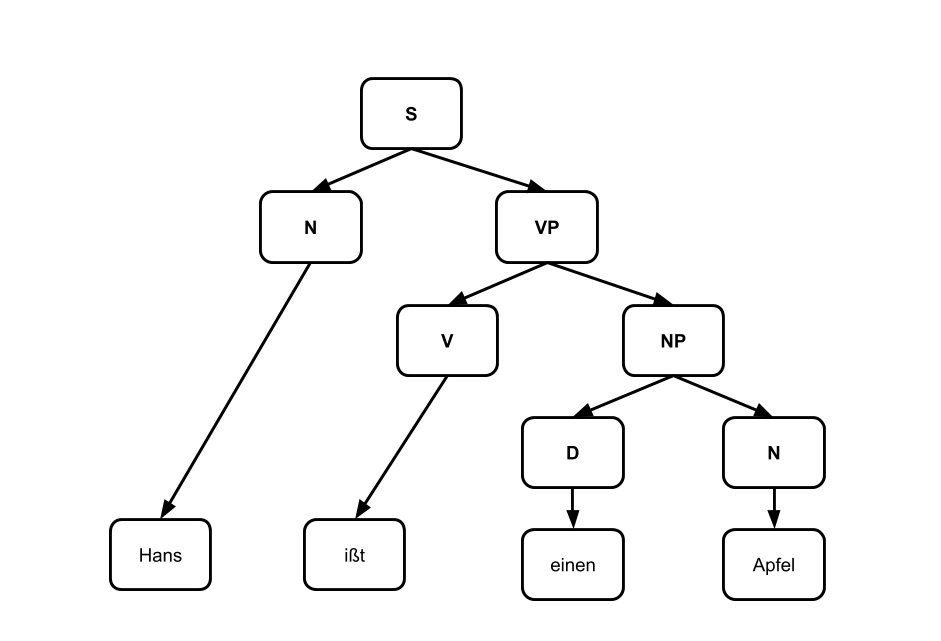
\includegraphics[width=\textwidth,height=8cm,keepaspectratio=true]
    {hans-eats-apples.png}
    \caption{
        An example parser tree
    }
    \label{fig:An example parser tree network}
\end{figure}

In this tree, the abbreviations S, D, N, V, NP, and VP refer to sentence, determinant, noun, verb, noun-phrase, and verb-phrase respectively. The words of the sentence are referred as leaf nodes of the tree: Hans, isst, einen and Apfel. The parts of speech (POS) tags associated with the above words are noun(N), verb(V), determinant(D), and noun(N) respectively. These are referred by the immediate parent of each word. The rest of the nodes are formed out of parsing. From the diagram, it is clear that the sentence followed three rules:

\begin{align*}
\textbf{S} \rightarrow \textbf{N} \, \textbf{VP} \\
\textbf{VP} \rightarrow \textbf{V} \, \textbf{NP} \\
\textbf{NP} \rightarrow \textbf{D} \, \textbf{N} 
\end{align*}
%Explanation about constituency parsing. How is it helpful

Jurafsky et al. \parencite{Jurafsky2008} in their 'Speech and Language processing' book stated that the parse tree is useful in many applications related to NLP. They are directly useful in grammar checking in word processing systems; a sentence that cannot be parsed is supposed to have grammatical errors. Most of the time, it is also an important intermediate representation for the semantic analysis of a sentence. Thus it plays an important role in applications such as relation extraction, semantic role labeling \parencite{Gildea:2002:NPP:1073083.1073124}, question answering and paraphrase detection \parencite{Callison-Burch2010}.

%A brief history of constituency parsing. 
  %Different languages - different parsing rules
  %Handwritten rules to Machine learning-based approach (statistical relationship)

%Penn Treebank dataset and SPMRL dataset  in state of parser in paper 'constituent parsing with a self-attentive encoder'
% Applying state of the art approach to a new dataset - %Tübingen data
In this thesis, we will apply state of the art techniques to perform constituent parsing for the German language.


% ----------------------------------------------------------------------------
\pagebreak
\section{Related work}

% FIND PAPERS FOR FOLLOWING
% Handwritten rules for parsing 
% probabilistic methods for context-free grammars
In the past, handwritten grammar played a central role in parsing. Context-free grammars (CFG) were used to model the rules and patterns of natural language. But given the complexity of a natural language, neither simple, broad-coverage grammar rules nor complex, constrained grammars were able to optimally accommodate sentences. A specific complex grammar with a lot of constraints was failing to parse a lot of sentences. At the same time, a simple and generic grammar was making it possible to have multiple ways of parsing even for a simple sentence. Statistical parsing systems offer a lot of possibilities of many rules to cope up with the flexibility of a language and at the same time has the predictive capabilities to figure out most likely parsing tree for a sentence. To build a statistical parsing system, the need for a versatile dataset is very critical. 

%There were considerable efforts put in by the research community to prepare large, standard and open datasets such as Wallstreet journal Penn treebank and SPGML, which is used as a standard benchmark to compare the algorithms. These datasets fuelled the research faster. 

Marcus et al.\parencite{Marcus1993} prepared the Penn Tree Bank dataset for the English language which consists of syntactic structures for sentences along with POS tags. It was revised multiple times and now it consists of more than 39,000 sentences with syntax trees and 7 million words with POS tags \parencite{Taylor2003}. This annotated information includes text from different sources such as IBM computer manuals, nursing notes, Wall Street Journal articles and transcribed telephone conversations. This served as a good corpus for building models to do parsing based on Machine Learning (ML). This leads to an empirical/data-driven approach to parsing than a rule-based approach. Some of the advantages of a treebank are reusability of a lot of other subsystems such as POS taggers, parsers, and a standard way to evaluate multiple parsing systems. 

Similarly, for the German language, Telljohann et al. \parencite{TubingenTreebank}, \parencite{Telljohann04thetuba} associated with the University of Tübingen, prepared a syntactically annotated German newspaper corpus TüBa-D/Z treebank. The annotations are done manually and consist of 3,816 articles, 104,787 sentences, and 1,959,474 tokens. It mainly distinguishes four levels of syntactic constituency: the lexical level, phrasal level, topological fields level, and clausal level. In addition to that, Brants et al. \parencite{Brants2002TheTT} also prepared a 35,000 syntactically annotated German newspaper sentences named TIGER treebank. It also contains different levels of annotation such as POS tags, phrase categories, and syntactic functions. These two data sources are very important in the field of NLP for the German language. 

%CFG-PCFG- Chart based CKY algorithm 
%Lexicalization of production rules
%Sudviding the categories - split based on closed grammar, horizontal markovization (binarization) and vertical markovization (parent categories), combination of latent models

Probabilistic context-free grammars (PCFG) \parencite{4569603} contains a probability score assigned to each production rule. These probabilities are assigned based on various methods and the simplest of it is considering the statistical properties of word combinations. They help to quantify the likelihood of different possibilities of parsing a sentence. The Chart based CKY \parencite{YOUNGER1967189} algorithm is a bottom-up parsing methodology that uses these probability scores to decide what combination of constituents is very likely. It only takes cubic time complexity rather than exponential by using dynamic programming techniques. 

The head word of a phrase gives a good representation of the phrase structure and meaning \parencite{Charniak_1997}. The Lexicalization of PCFG \parencite{charniak2000} will create more rules of specific cases and the probability scores can be trained for each production rule. This indeed improves the accuracy of parsing, but it increases production rules exponentially which results in sparseness. Kelin and Manning \parencite{kleinunlexical} found that lexicalized PCFG does not capture lexical selection between content words but just basic grammatical features like verb form, verbal auxiliary, finiteness, etc. This kind of splitting can be done horizontally while binarizing the tree and vertically by parent annotation. It achieved 85.7\% F1 score and does not lead to too many production rules but at the same time captures the essence of context. Until now the rules of grammar were handwritten which were picked carefully by experts. Petrov and Klein \parencite{petrov2006} came up with an unsupervised ML approach that uses base categories and learns subcategorizing and splitting using treebank data. They used expectation maximization (EM) algorithm, like Forward-Backward for HMMs but constrained by a tree structure and achieved 90.2\% F1 score. 

On the other hand, neural networks have been raising and becoming a prominent architecture to build machine learning (ML) systems. They were giving state of the art results for many NLP applications. They are also used to develop a better alternative for the representation of words or other features of text. 

% Recursive neural network
The constituent parsing of a given sentence involves outputting a tree which is fundamentally made of recursive structures of branches or merges of words or phrases. Socher et al. [\parencite*{RichardSocher2011}, \parencite*{Socher}, \parencite*{Sochera}] implemented a neural network-based parsing which is specialized in learning recursive structures in a sentence and simultaneously learning compositional vectors for phrases. Their work achieved an accuracy of 90.4\% F1 score and it is 20\% faster than Stanford factored parser. The system involves two bottom-up parsing; the first parsing done by a base Probabilistic Context-Free Grammar(PCFG) parser using CKY dynamic programming and select 200 best parses; the second pass is done by their best recursive neural network model with expensive matrix calculations on those 200 best results. 

%Encoder-Decoder artchitecture
%Encoder - FeedForward neural network, CNN, RNN , Bi-RNN,
%\parencite*{Vaswani2017}
%\parencite*{Stern2017}
%\parencite*{Gaddy2018}

Stern et al. \parencite*{Stern2017} implemented a minimum span neural network-based constituency parser and achieved an accuracy of 91.79\% F1 score on Penn Treebank dataset. They used an encoder-decoder architecture where the encoder converts the input into a different representation with context information and the decoder uses this augmented information to build the tree and get trained to become better. Bi-directional RNN with LSTM \parencite{schuster1997} modules were used to encode the words in a sentence. This encoding gives out two vectors for each word containing the sentential context from the left and right direction. This encoded output is used by two independent scoring systems; one to label the span and the other to choose the split. Their research work involved experimenting with the above computed encoded output with chart-based bottom-up and greedy top-down parsing. Surprisingly the results of using top-down with run time complexity $O(n^2)$ is as good as using a bottom-up approach wherein a global optimized tree is chosen with run time complexity $O(n^3)$. The bottom-up parsing was making decisions at every stage with the already computed values for the whole tree beneath; whereas the top-down parsing can refer to only local information. These results credit the ability of bi-directional RNN modules in capturing a lot of complex relations among words in a sentence. By using rich and expressive word vector representations, the encoding and decoding architectures are made simpler. 

%Encoder - self-attention module
Kitaev et al. \parencite*{Kitaev2019} also implemented an encoder-decoder based neural network architecture for constituency parsing and they achieved state of the art accuracy of 95.13\% F1 score on Penn Treebank dataset. Their parser also outperforms all the previous parsers on 8 of the 9 languages in SPMRL dataset which includes German. In this, instead of LSTM modules, attention modules \parencite*{Vaswani2017} are used. Attention modules are better in expressing how two sentences or inputs are relevant to each other by expressing them in a matrix with columns and rows as words/components of sentences/inputs of each. At the same time, attention modules can also be applied to a sentence itself to express which part of the sentence is dependent on which other words. These capture the relationships of words in a sentence among themselves. Several self-attention modules are used in combination to encode the information and context in each sentence. The use of attention makes explicit how information is propagated between different locations in the sentence. A chart-based decoder implemented by Stern et al. \parencite*{Stern2017} is used along with the modifications from Gaddy et al \parencite*{Gaddy2018}. They also found that positional information plays a very important role in parsing and inclusion of ELMo(Embeddings from Language Models) improved their accuracy by 3\%. 

%Papers to write about:
%Decoder - chart-based, greedy or beam search. top-down and bottom-up

%Parser showdown at the Wallstreet corral: An empirical investigation of error types

%Parsing three german treebanks: Lexicalized and Unlexicalized Baselines


% ----------------------------------------------------------------------------
\pagebreak
\section{Background Study}
 In this thesis, we develop a neural network based constituent parser for the German language. The required information to understand the different components of the proposed system is explained briefly in this section. 

\subsection{Neural networks and its components}

Recently, neural networks have become the most popular approach for building machine learning systems. Neural networks compose many interconnected, fundamental, functional units called neurons. They are loosely inspired from the field of neuroscience. There are different ways by which these neurons can be networked with each other. That defines its ability to learn. 

\begin{figure}[H]
    \centering
    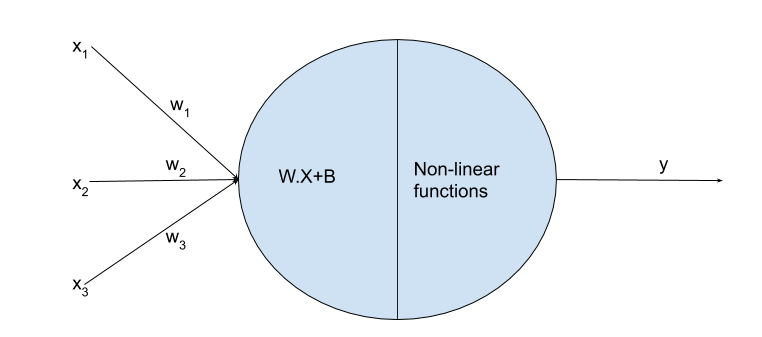
\includegraphics[width=\textwidth,height=8cm,keepaspectratio=true]
    {single-neuron.png}
    \caption{
        Single Neuron
    }
    \label{fig:single_neuron}
\end{figure}

Each neuron in the network takes in multiple scalar inputs and gives out a scalar output. It uses parameters (weights and bias) to perform linear transformation of the input and most often applies non-linear function subsequently.

The important components of any machine learning approach are model, data, loss function, and optimizer. The model defines the architecture of system, data helps the model to get trained, loss function helps the system to understand how has it performed during its learning, and optimizer helps the system to fine-tune its parameters of model to get better results.

\subsubsection{Feed-forward network}

There are different architectures of neural networks that vary mostly in how the neurons are connected and how the weights are managed. Feed-forward neural network \parencite{Svozil1997} is a basic neural network architecture which arranges neurons in layers that reflect the flow of information. They are used to perform supervised machine learning wherein label data regarding classification is mandatory. These networks should contain an input layer that takes in data and an output layer which represents prediction of classification. It can have one or many hidden layers and each neuron in one layer is connected with every other neuron in the subsequent layer as given in Figure \ref{fig:Feed forward neural network}

\begin{figure}[htpb]
    \centering
    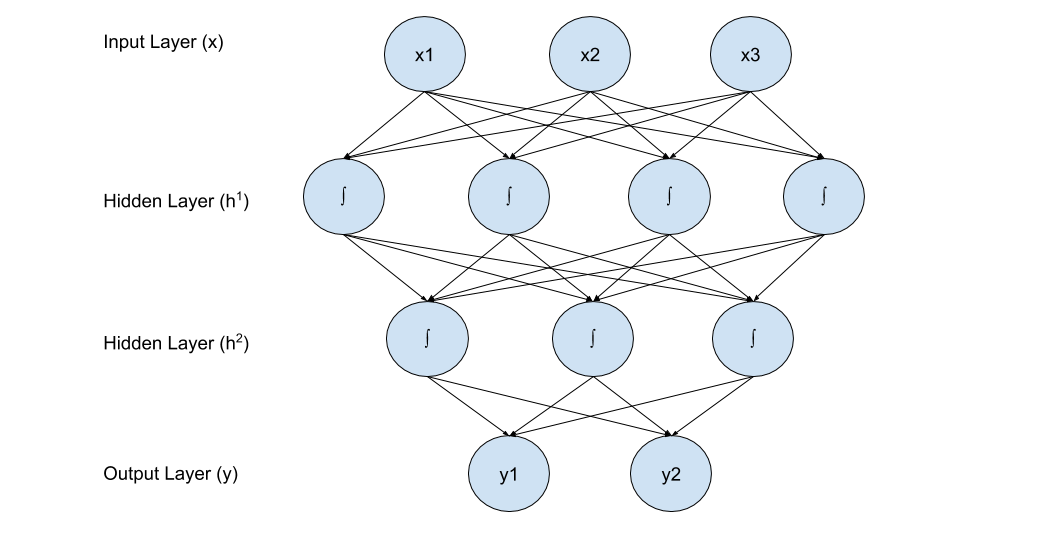
\includegraphics[width=\textwidth,height=8cm,keepaspectratio=true]
    {feed-forward-neural-network.png}
    \caption{
        A Feed-Forward neural network.
    }
    \label{fig:Feed forward neural network}
\end{figure}

There are 4 layers in figure \ref{fig:Feed forward neural network}. Each circle is a neuron with incoming lines as inputs and outgoing lines as outputs to the next layer. Each line carries weight and the input layer has no weights since it has no incoming lines. The input layer consists of 3 neurons and the extracted features of raw data will be sent through these neurons. The first hidden layer consists of 4 neurons, of which each neuron takes 3 inputs from input layer. Each input to the neuron in the first hidden layer is multiplied by a unique weight variable and added together.  Finally, the output is added with a bias variable and will be passed to a non-linear activation function as shown in equation \ref{equ: feed forward hidden layer}. The same process is carried out for the second hidden layer except that it has 3 neurons and each neuron will take 4 inputs from the first hidden layer. The output layer consists of 2 neurons and each will take 3 inputs from the second hidden layer as shown in equation \ref{equ: feed forward output layer}.

\begin{equation} \label{equ: feed forward hidden layer}
h^1 = g^1(xW^1 + b^1)
\end{equation}

\begin{equation}
h^2 = g^2(h^1W^2 + b^2)
\end{equation}

\begin{equation} \label{equ: feed forward output layer}
\mathrm{NN_{MLP2}}(x) = y = g^3(h^2W^3 + b^3)
\end{equation}
\begin{align*}
x \in \mathbb{R}^{d_{in}}, y \in \mathbb{R}^{d_{out}} \\
W^1 \in \mathbb{R}^{d_{in} \times d_1}, b^1 \in \mathbb{R}^{d_1}, h1 \in \mathbb{R}^{d_{1}} \\
W^2 \in \mathbb{R}^{d_1 \times d_2}, b^2 \in \mathbb{R}^{d_2}, h2 \in \mathbb{R}^{d_{2}}\\
W^3 \in \mathbb{R}^{d_2 \times d_\mathrm{out}}, b^3 \in \mathbb{R}^{d_{out}}
\end{align*}

Here $\mathbf{W^1, W^2, W^3}$,  and $\mathbf{b^1}$, $\mathbf{b^2}$ and $\mathbf{b^3}$ are matrices and bias vectors for first, second and third linear transforms, respectively. The functions $g^1$, $g^2$ and $g^3$ are activation functions and they are almost always non-linear. With respect to figure~\ref{fig:Feed forward neural network}, the values of $d_\mathrm{in}$, $d_{1}$, $d_{2}$ and $d_\mathrm{out}$ are 3, 4, 3, and 2, respectively. 

\subsubsection{Training a neural network}

Training is an essential part of learning and like many supervised algorithms, a loss function is used to compute the error for the predicted output against the actual output. The gradient of the errors is calculated with respect to each weight and bias variable by propagating backward using the chain rule of differentiation. The values of the weights and bias are adjusted with respect to the gradient and a learning parameter. Typically a random batch of inputs is selected and a forward pass is carried out which involves multiplying weights, adding bias and applying an activation function to predict outputs. The average loss is computed for that batch and the parameters are adjusted accordingly. This optimization technique is called stochastic gradient descent \parencite{Bottou2012}. A number of extensions exist, such as Nesterov Momentum \parencite{Sutskever2013} or AdaGrad \parencite{Duchi2011}. Some loss functions that exist are hinge loss (binary and multiclass), log loss and categorical cross-entropy loss \parencite{Goldberg2016}. 

%\begin{align*}
%L_{hinge(binary)}(\hat{y},y) = max(0,1-y.\hat{y})
%\end{align*}

The categorical cross-entropy loss is used when predicted output refers to a probability distribution. This is typically achieved by using a softmax activation function in the output layer. Let $y = y^{1}, y^{2}, \dots, y^{n}$ be representing the target multinomial distribution over the labels $1,2,\dots,n$ and let $ \hat{y} = \hat{y}_{1},\hat{y}_{2},\dots,\hat{y}_{n}$ be the network's output which is transformed by a softmax function. The categorical cross-entropy loss measures the difference between the true label distribution $y$ and the predicted label distribution $\hat{y}$. 
\begin{align*}
L_\mathrm{cross-entropy}(\hat{y},y) = -\sum_iy_i \cdot \log(\hat{y_i})
\end{align*}

For hard classification, $y$ is a one-hot vector representing the true class. Here $t$ is the correct class assignment. Training will attempt to set the correct class $t$ to 1 which inturn will decrease the other class assignment to 0.
\begin{align*}
L_{\mathrm{cross-entropy(hard classification)}}(\hat{y},y) = -\log(\hat{y_t})
\end{align*}

The overfitting in neural networks will cause the trained system to perform well only for trained data but not on the test data. This can be minimized by using regularization techniques such as $L_2$ regularization and dropout \parencite{Hinton2012}. $L_2$ regularization works by adding a penalty term equal to sum of the squares of all the parameters in the network to the loss function which is being minimized. Dropout, instead, works by randomly ignoring half of the neurons in every layer and corrects the error only using the parameters of another half of neurons. This helps to prevent the network from relying on only specific weights.

\subsubsection{Activation Functions}

The activation functions help the neural network models to approximate any nonlinear function. Different activation functions have different advantages. Some popular activation functions are sigmoid, hyperbolic tangent and rectifiers \parencite{Goldberg2016}:

\begin{enumerate}

\item The sigmoid activation function is a S-shaped function which transforms any value into the range between $0$ and $1$.  
\begin{align*}
\sigma (x) = \frac{1}{1 + e^{-x}}
\end{align*}

\item The hyperbolic tangent function is also a S-shaped function, but it transforms any value into the range between $-1$ and $1$.
\begin{align*}
\tanh (x) = \frac{e^{2x}-1}{e^{2x}+1}
\end{align*}

\item The rectifier activation function clips values lesser than $0$
\begin{align*}
\mathrm{ReLU}(x) = \mathrm{max}(0,x)
\end{align*}

\end{enumerate}

The sigmoid activation function is not used in internal layers of neural networks since other functions have been giving better results empirically. The rectifier activation function is commonly used since it performs faster and better than sigmoid and hyperbolic tangent functions. Instead of an activation function, the function in output layer $g^3$ can be a transformation function such as softmax to convert values to represent a discrete probability distribution. Each of the converted values will be between $0$ and $1$ and sum of all of them will be $1$.

\begin{align*}
y = \begin{bmatrix} y_1 & y_2 & \dots & y_k \end{bmatrix} \\
s_i = \mathrm{softmax(y_i)} = \frac{e^{y_i}}{(\sum_{j=1}^ke^{y_j})}
\end{align*}

\subsection{Convolution Neural networks}

Feed-forward networks do not take into account the order of input and so they are not good at representing text data. According to it, words $w_i$ and $w_j$ are independent and do not influence each other. 
Convolution neural networks \parencite{lecun-bengio-95a}evolved initially in the vision community where they showed tremendous success in object detection regardless of position in an image. For an image, convolutions are 2-dimensional matrix whereas for text it is implemented by a 1-dimensional vector. These are slid over the input taking into account of their spatial dependencies, resulting in capturing the local important characteristics irrespective of its location in the input. These are then fed into a pooling layer which combines all these characteristics computed from different convolutions either by taking maximum or average of them.

\begin{figure}[H]
    \centering
    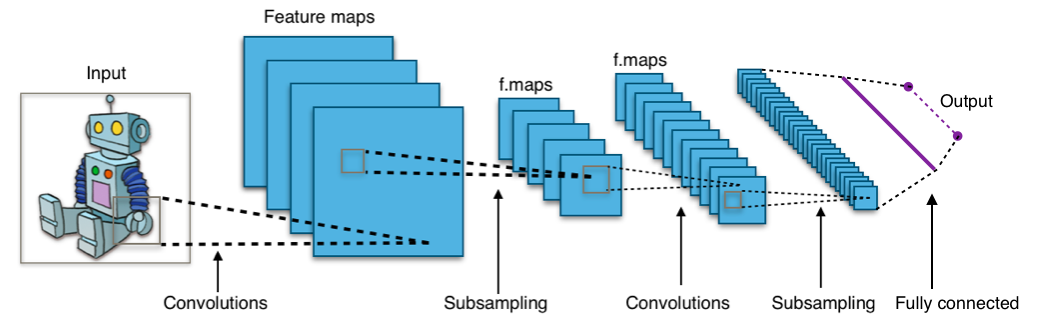
\includegraphics[width=\textwidth,height=6cm,keepaspectratio=true]
    {cnn-1.png}
    \caption{
        CNN architecture \parencite{cnn-1}
    }
    \label{fig:CNN architecture}
\end{figure}

In figure \ref{fig:CNN architecture}, many 2-dimensional convolutional filters are slid over X and Y axes of an input which is a robot image. It outputs a 3-dimensional tensor whose dimensions are influenced by the number and dimensions of filters and length of stride. This output captures many local features of an image and each one is represented by a matrix. This is followed by a max-pooling layer which filters the features by allowing only the most dominant ones. This combination of convolution and pooling is applied many times and finally passed onto a feed-forward network with softmax at the end. 

In the case of text data, convolutional filters are 1-dimensional and they are applied over a k-word sliding window. Convolution neural networks consider ordering to some extent based on the value of k which helps to capture local dependencies. In figure \ref{fig:Char CNN architecture}, words in a sentence is referred as $x_0, x_1, \dots, x_n$; the value of k is 2 and so it convolves consecutive words. It is then passed to neural network module and the outputs $y_0, y_1, \dots, y_n$ are obtained. Each vector $y_i$ embodies the context of $x_i$ and $x_{i+1}$. If each of the characters in a word is represented by a vector then a 2-dimensional convolutional filter can be used and this will be same as convolutions applied on a image.
\begin{figure}[H]
    \centering
    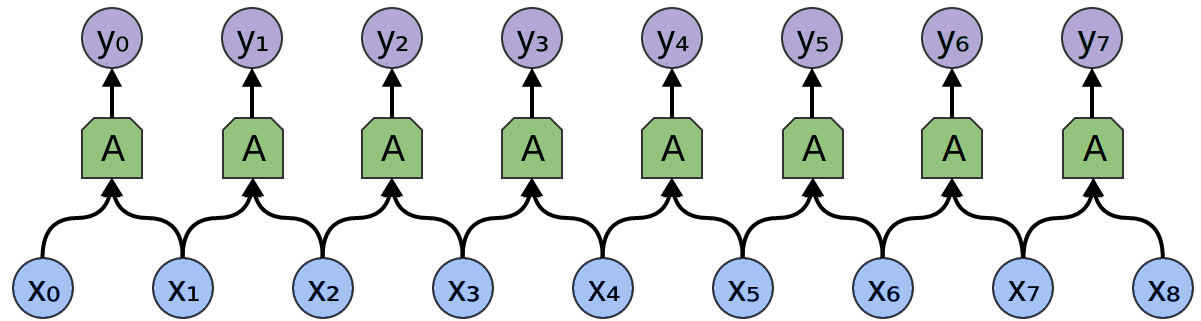
\includegraphics[width=\textwidth,height=6cm,keepaspectratio=true]
    {cnn-2.png}
    \caption{
        CNN architecture on words
    }
    \label{fig:Char CNN architecture}
\end{figure}


\subsection{Recurrent Neural networks}

% Relation with conditional probabilities

For text data, the input is sequential and of unknown length, where the ordering of words is important. Techniques such as continuous bag of words \parencite{DBLP:journals/corr/abs-1301-3781} can be used with feed-forward networks to convert sequential input into fixed-length vectors but it will discard the order of words. Convolutional neural networks (CNN) \parencite{Bengio1997} are good at capturing the local characteristics of data irrespective of its position. In this, a nonlinear function is applied to every $k$-word sliding window and captures the important characteristics of the word in that window. All the important characteristics from each window are combined by either taking maximum or average value from each window. This captures the important characteristics of a sentence irrespective of its location. However, because of the nature of CNNs, they fail to recognize patterns that are far apart in the sequence.

Recurrent neural networks (RNN) accept sequential inputs and are often able to extract patterns over long distances \parencite{Elman}. A RNN takes input as an ordered list of input vectors $\mathrm{\mathbf{x_1},\dots,\mathbf{x_n}}$ with initial state vector $\mathbf{h_0}$ and returns an ordered list of state vectors $\mathrm{\mathbf{h_1},\dots,\mathbf{h_n}}$ as well as an ordered list of output vectors $\mathrm{\mathbf{o_1},\dots,\mathbf{o_n}}$. At time step $t$, a RNN takes as input a state vector $\mathbf{h_{t-1}}$, an input vector $\mathbf{x_{t}}$ and outputs a new state vector $\mathbf{h_{t}}$ as shown in figure \ref{fig:A basic RNN architecture}. The outputted state vector is used as input state vector at the next time step. The same weights for input, state, and output vectors are used in each time step.  

%RNN - architecture, how does it support the sequence, (Elman, 1990) 
%Back Propagation through time (BPTT) - (Werbos, 1990) \parencite{Werbos1990}
%Long distance dependencies - LSTM and GRU (Hochreiter and Schmidhuber 1997) and (Cho et al.)
%(did not find the citation for GRU) \parencite{Hochreiter1997}
%Recursive Neural Networks - for syntactic structure (trees ) (pollack 1990; socher, manning and ng 2010) \parencite{Pollack1990} \parencite{Socher}

\begin{figure}[htpb!]
    \centering
    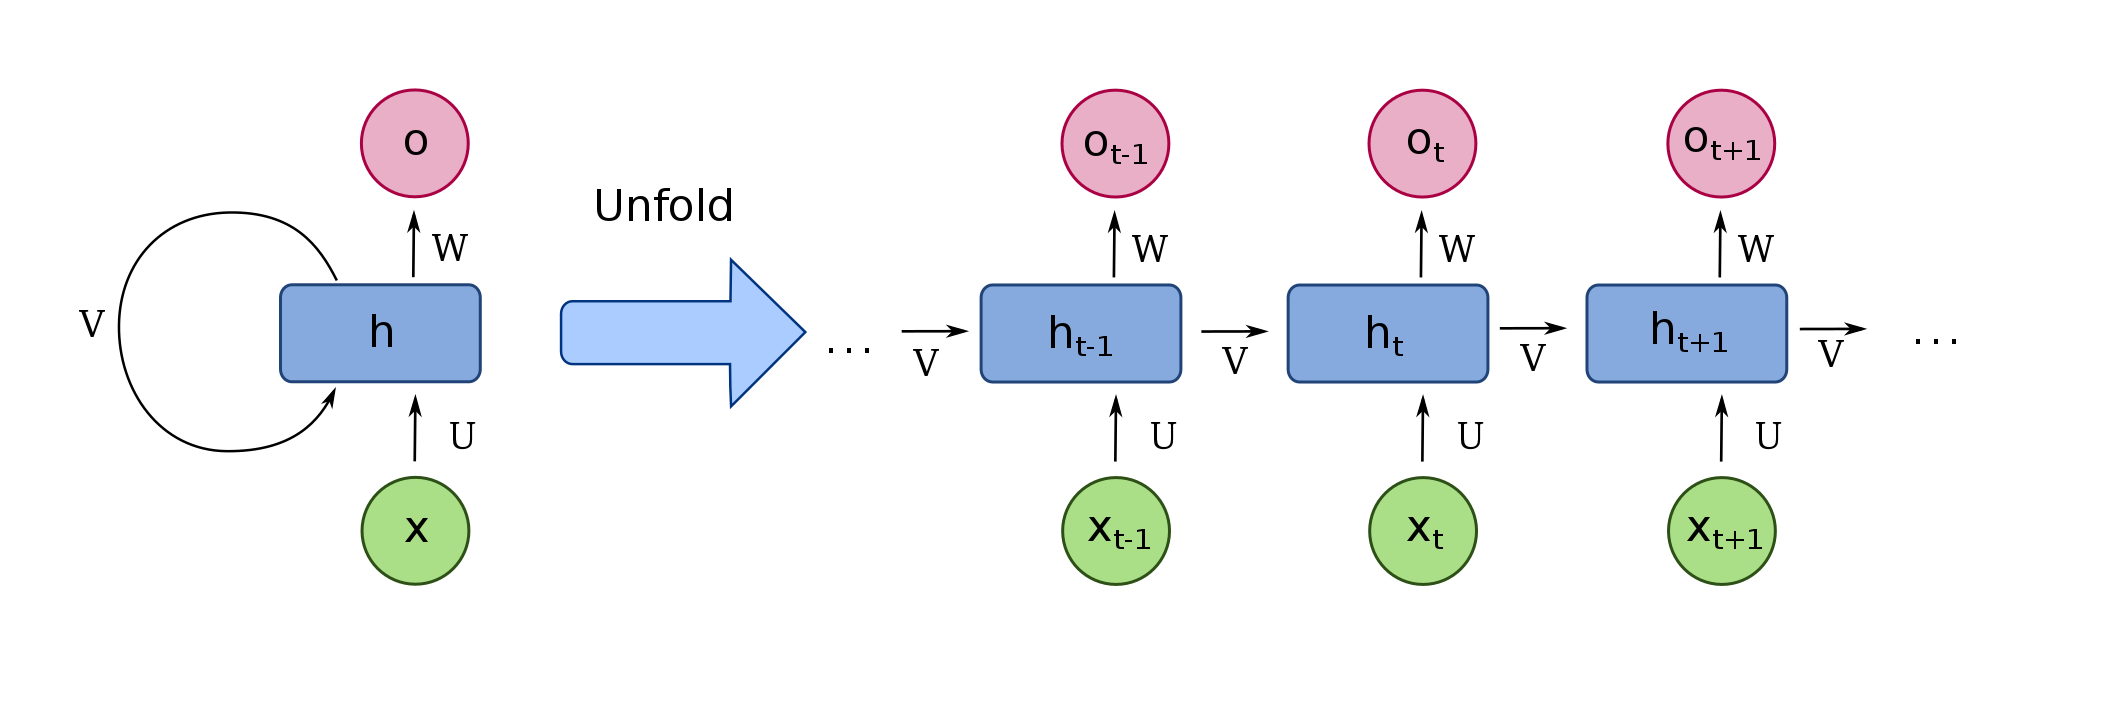
\includegraphics[width=\textwidth,height=6cm,keepaspectratio=true]
    {Recurrent_neural_network_unfold.png}
    \caption{
        A basic example of RNN architecture \parencite{rnn-1}.
    }
    \label{fig:A basic RNN architecture}
\end{figure}

\begin{align*}
\mathrm{RNN}(h_0,x_{1:n}) = h_{1:n}, o_{1:n} \\
h_i = g^1(h_{i-1}V + x_iU + b^1) \\
o_i = g^2(h_iW + b^2) 
\end{align*}

\begin{align*}
x_i \in \mathbb{R}^{d_x}, U \in \mathbb{R}^{d_x \times d_h} \\
h_i \in \mathbb{R}^{d_h}, V \in \mathbb{R}^{d_h \times d_h}, b^1 \in \mathbb{R}^{d_h} \\
o_i \in \mathbb{R}^{d_o}, W \in \mathbb{R}^{d_h \times d_o}, b^2 \in \mathbb{R}^{d_o}
\end{align*}

Here the functions $g^{1}$ and $g^{2}$ are non-linear activation functions; $\mathbf{W}$, $\mathbf{V}$, and $\mathbf{U}$ are weight matrices and $\mathbf{b^{1}}$, $\mathbf{b^{2}}$ are bias vectors. 

To train a RNN, the network is unrolled for a given input sequence and the loss function is used to compute the gradient of error with respect to parameters involved in every time step by propagating backward through time. After that, the parameters are adjusted to reduce the error in prediction \parencite{Werbos1990}. 

\subsection{LSTM}

While training RNNs, a common problem that especially occurs with long input sentences is that the error gradients might vanish (become too close to zero) or explode (become too large) which results in numerical instability during the backpropagation step. The gradient explosion can be handled by clipping a given gradient when it goes beyond the threshold. LSTM networks \parencite{Hochreiter1997} solve the vanishing gradient problem by introducing memory cells that are controlled by gating components. These gating components decide at each time step, what parts of the hidden state should be forgotten and what parts of new input should be included in the memory cells. These memory cells are involved in the computation of hidden states, which in turn are used to compute the output states. This technique has been shown to provide good results in practice, in capturing the dependency between words even though separated by a long distance.

\begin{figure}[htpb!]
    \centering
    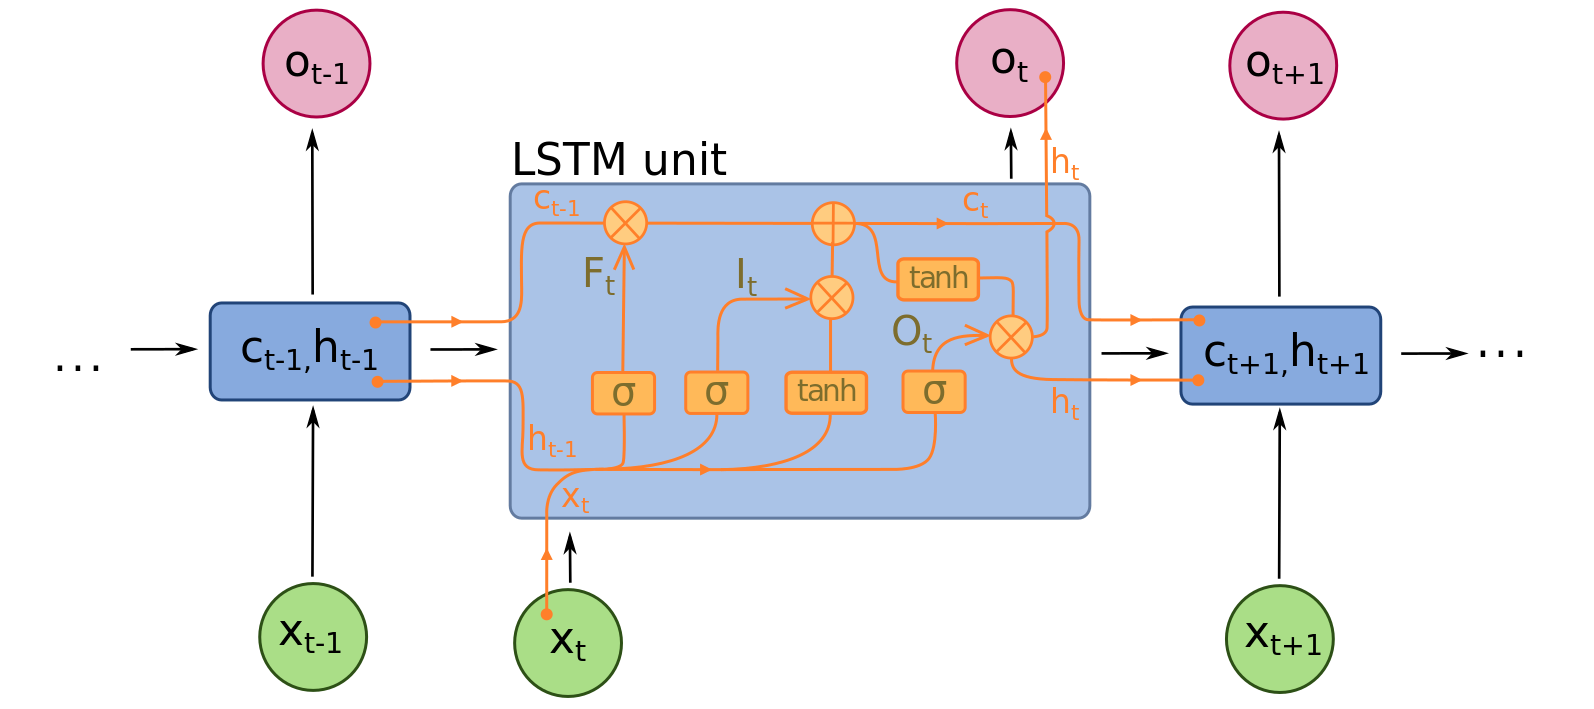
\includegraphics[width=\textwidth,height=6cm,keepaspectratio=true]
    {lstm-1.png}
    \caption{
        LSTM architecture \parencite{rnn-2}.
    }
    \label{fig:LSTM architecture}
\end{figure}

\begin{align*} \label{lstm_equation}
s_j = R_{LSTM}(s_{j-1},x_j) = [c_j;h_j] \\
c_j = c_{j-1} \odot f + g \odot i \\
h_j = tanh(c_j) \odot o \\
i = \sigma(x_jW^{xi} + h_{j-1} W^{hi}) \\
f = \sigma(x_jW^{xf} + h_{j-1} W^{hf}) \\
o = \sigma(x_jW^{xo} + h_{j-1} W^{ho}) \\
g = \sigma(x_jW^{xg} + h_{j-1} W^{hg}) \\
y_j = O_{LSTM}(s_j) = h_j \\
s_j \in \mathbb{R}^{2.d_h},   x_i \in \mathbb{R}^{d_x},  c_j,h_j,i,f,o,g \in \mathbb{R}^d_h, \\
W^{xo} \in \mathbb{R}^{d_x*d_h},  W^{ho} \in \mathbb{R}^{d_h*d_h}
\end{align*}

Here the symbol $\odot$ denotes component-wise product. The LSTM uses 3 gating components such as input gate (i), forgot gate (f) and output gate (o) respectively. They contain a sigmoid function to convert the values between 0 and 1 which is used to decide how much to keep. The memory cell state c\textsubscript{j} is obtained by controlling the previous memory cell state with forgot gate and the new input state (g) with input gate. The obtained memory cell state is controlled by the output gate to get the hidden state h\textsubscript{j}.

A similar type of architecture with fewer elements is also effective in handling long-range dependencies is Gated Recurrent Unit (GRU) \parencite{cho2014learning}.

\subsection{Bidirectional RNN}
A RNN computes the state of current word $\mathbf{x_{i}}$ only based on the words in the past, i.e. $\mathrm{\mathbf{x_1},\dots,\mathbf{x_{i-1}}}$. However, the following words $\mathrm{\mathbf{x_{i+1}},\dots,\mathbf{x_{n}}}$ will also be useful in computing the hidden state regarding the current word. The bidirectional RNN (biRNN) \parencite{bidirectionalRNN} solves the problem by having two different RNNs. The first RNN is fed with the input sequence $\mathrm{\mathbf{x_{1}},\dots,\mathbf{x_{n}}}$ and the second RNN is fed with input sequence in reverse. The hidden state representation $\mathbf{h_{i}}$ is then composed of both the forward and backward states. Each state representation consists of the token information along with sentential context from both directions which has shown better results than classical uni-directional RNNs in practice.

\begin{figure}[H]
    \centering
    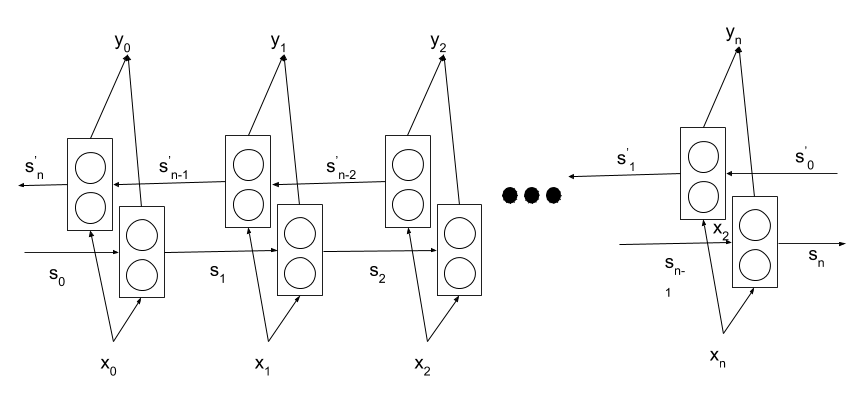
\includegraphics[width=\textwidth,height=10cm,keepaspectratio=true]
    {bi-directional-rnn-1.png}
    \caption{
        Bidirectional RNN
    }
    \label{fig:bi-directional-rnn-1.png}
\end{figure}

\subsection{Data Representation}

The representation of data is a very important factor in improving the performance of any machine learning application. In the past, inputs are differentiated using sparse vectors called one-hot vectors. If there are $n$ inputs then there will be  $n$ one-hot vectors and each of its dimension will be $n$. The input $w_i$ will be represented by a vector whose elements will be 0 except that the value of $i^{th}$ element to be 1. Each input is orthogonal to all others and the larger the number of inputs the higher the dimensions of vectors. It also increases the sparsity of representation which is a disadvantage. 

\subsubsection{Word embeddings}

Instead of representing each word by a vector of dimension $n$ that is equal to the total number of words in a training dataset, a dense vector of dimension $d$ where $d << n$ is used. The difference here is that all the elements of vector can have any values whereas with one-hot vectors it is mostly 0 except one element with value 1. Unlike one-hot vectors, these dense vectors will be initialized randomly at the beginning and will be trained according to the application needs. These dense vectors are called as word embeddings. The dimensionality of these word embeddings typically ranges from 50 to few hundreds. 

There are two advantages of using word embeddings and they are listed here:
\begin{enumerate}
\item Computation becomes efficient. It consumes less space and so the parameters that deal with will also get reduced. With the ability to have any values for each element, the representation becomes efficient
\item Model training will make the dense vectors to have similar values for similar features. This will make the training efficient
\end{enumerate}

Many NLP applications were benefitted using word embeddings and they are initially made popular by few works. \parencite{10.5555/944919.944966}, \parencite{Schwenk2006}. 

There are many unsupervised learning approaches to compute word embeddings and the most common ones are word2vec \parencite{mikolov2013efficient}, and Glove \parencite{pennington2014glove}. These pre-trained word embeddings can be used directly or word embeddings with random initialization can be learned while performing task specific training. 

Mikolov et al. analyzed these dense vectors and figured out that they posses good syntactic and semantic word relationships \parencite{mikolov2013linguistic}. For instance the vector calculation $v_{madrid} - v_{spain} + v_{france}$ is closer to $v_{paris}$.  This shows that it captures the capital to city relationship effectively. Similarly man to woman, company to ceo, city to zip code, and compartive to superlative are captured very well. This shows that dense vectors inherently embodies relationship attributes. They are much more than mere numbers. The figure \ref{fig:word_properties} is an illustration of embeddings representing words such as man, woman etc. The relationship between man and woman, uncle and aunt, and king and queen are captured by similarity in the results of those vector calculations.

\begin{figure}[H]
    \centering
    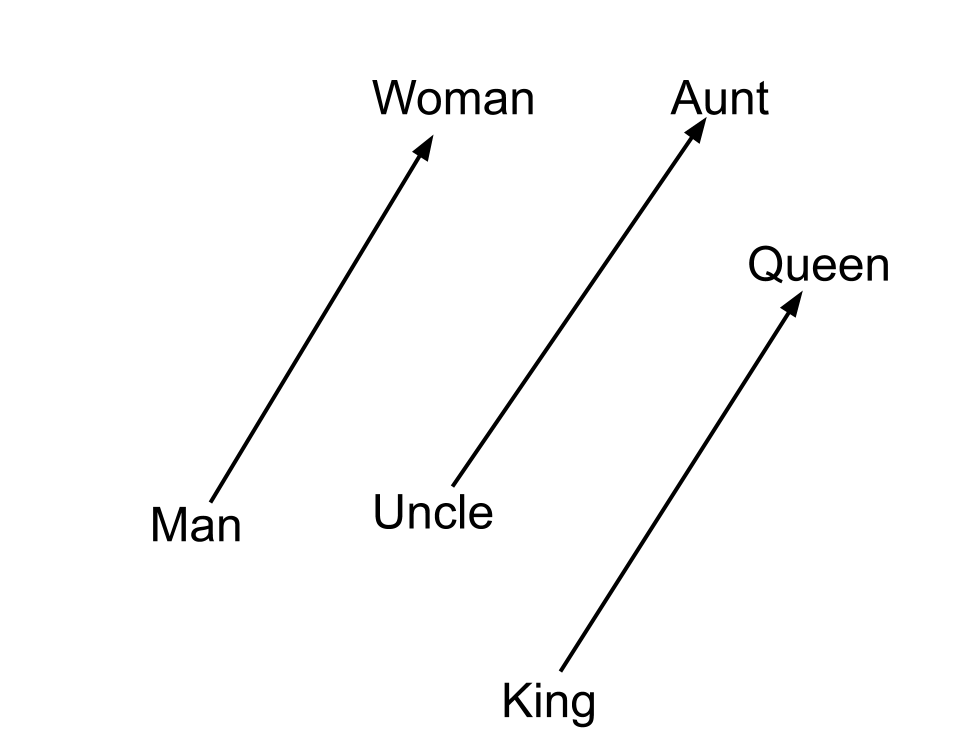
\includegraphics[width=\textwidth,height=10cm,keepaspectratio=true]
    {word2vec-gender-relation.png}
    \caption{
        Word embeddings charcteristics
    }
    \label{fig:word_properties}
\end{figure}


The word embeddings can be built over character embeddings. The representation of words can be built using convolutional network over the words \parencite{dos2014deep}. Also the word vectors can be computed using final states of bi-directional RNN over the characters in a word \parencite{ling-etal-2015-finding}. Character embeddings compose syntactic relations as the character patterns within words are strongly related to their syntactic function \parencite{Goldberg2016}.Some advantages of character embeddings are the models are smaller in size since only one vector for each character and also it is possible to compute a vector for any word irrespective of its presence in training dataset. 

\subsubsection{Embeddings from Language Models (ELMo)}
Word sense is one of the meanings of a word. Words have different meanings depending on the context it is being used. The disadvantage of word embeddings are that it uses only one vector to represent all word 
senses of a word.  Say for e.g., consider the sentences below:
\begin{itemize}
\item We went to see the $play$ Romeo and Juliet
\item The children went out to $play$ in the park
\end{itemize}
Here the word $play$ means different in each of the sentences. But with word embeddings, during both the times same vector will be used to represent it. 

Peter et al. \parencite{peters2018deep} created a deep contextualized word representation which models:
\begin{itemize}
\item Complex characteristics of the word use
\item how these uses vary across many context                   
\end{itemize}

The representation is so powerful that it significantly improves six challenging NLP applications such as question answering, textual entailment, and sentiment analysis. The figure \ref{fig:ELMO} shows the architecture of model which produces ELMo based representations. This involves training for a longer period of time on a very large corpus.

\begin{figure}[H]
    \centering
    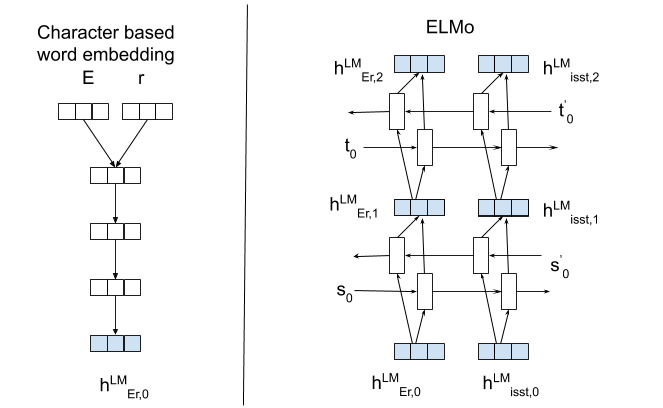
\includegraphics[width=\textwidth,height=10cm,keepaspectratio=true]
    {elmo-1.png}
    \caption{
        ELMo
    }
    \label{fig:ELMO}
\end{figure}

Character embeddings with convolution filters or bidirectional RNNs are used to represent words as shown in the left side of above figure. These representations are passed through a two layered bidirectional RNNs and the outputs for a word $w_i$ are $h^{LM}_{w_{i},1}$ and $h^{LM}_{w_{i},2}$. Since it involves RNN, the vectors for word $w_i$ will be dependent on the previous words. The training for producing ELMo embeddings is based on an unsupervised language modeling task. In this, for a sentence,  when $w_i$ is passed as input, the system predicts the next word $w^p_{i+1}$ given the previous words. In the next state, the actual word $w_{i+1}$ is passed as input and now the system predicts next word. In the case of ELMo, these predicts happen at the final layer which is at $h^{LM}_{w_{i},2}$. This models the behavior of conditional probability given by $P(w_i|w_ {i-1},w_{i-2},...w_1)$.

The embeddings for words are obtained by considering all three layers. For every task, for every word, the system is trained to extract embeddings from all three layers using a weighted average of them. The following equation shows how to extract embeddings:
\begin{align*} 
{ELMo}^{task}_k = \gamma^{task} \sum_{j=0}^{2} s^{task}_j h^{LM}_{k,j}
\end{align*}

In this $\gamma^{task}$ is the scalar that scales all vectors and $s^{task}_j$ is the scalar weight for each layer representation with $s^{task}_j \epsilon [0,1]$ and $\sum_{j=0}^{2} s^{task}_j = 1$. 

The following table captures the difference between the outputs of GloVe and ELMo for the word 'play'. The nearest neighbor is calculated using eucledian distance and for Glove they are playing, game, games etc which is quite general. Whereas for ELMo, it is quite specific and very context rich. 

\begin{figure}[H]
    \centering
    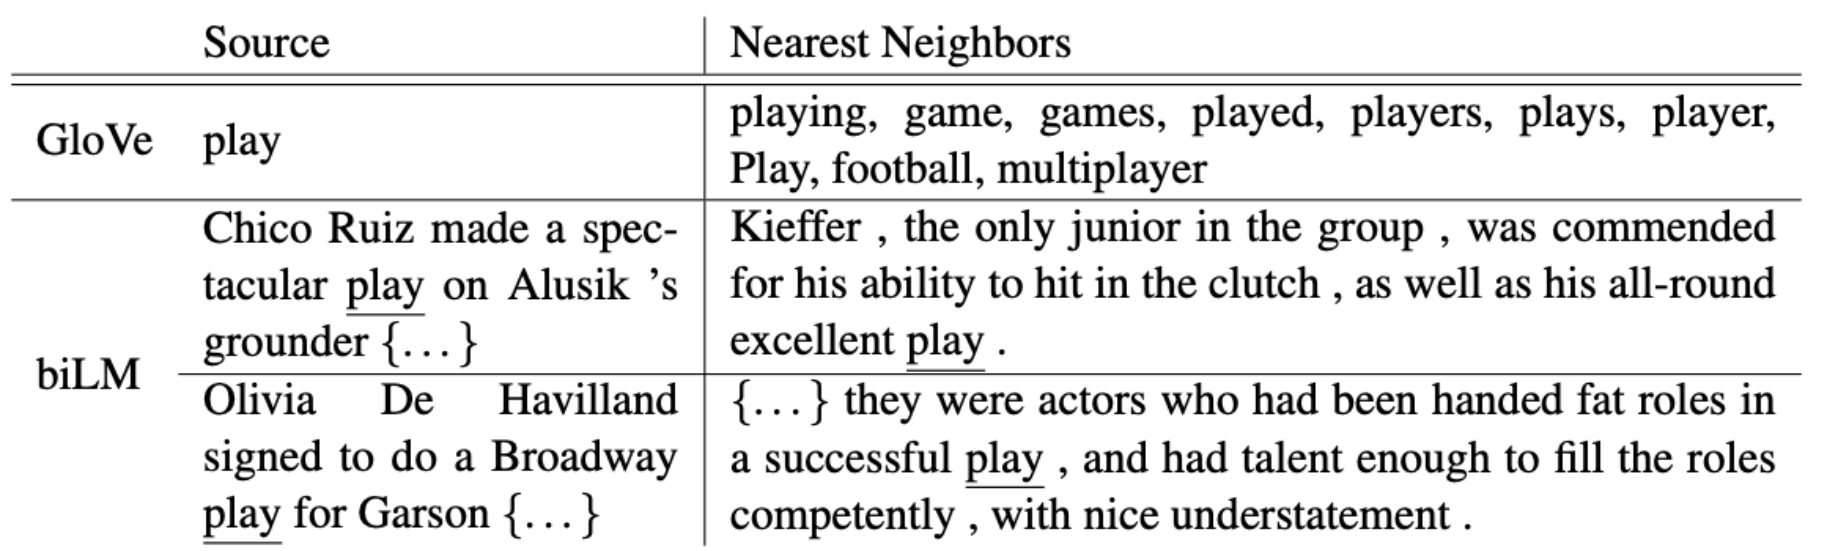
\includegraphics[width=\textwidth,height=10cm,keepaspectratio=true]
    {elmo-2.png}
    \caption{
        ELMo analysis \parencite{GerElmo}
    }
    \label{fig:ELMO2}
\end{figure}
\subsection{Attention}

%Talk about translation in general
%How does this weightage help
%Accuracy improvements
\parencite{bahdanau2014neural}

Attention models were first introduced in machine translation system \parencite{bahdanau2014neural}. Machine translation system were implemented using only sequence to sequence architectures which predominantly uses RNN networks \parencite{sutskever2014sequence}. 

\begin{figure}[H]
    \centering
    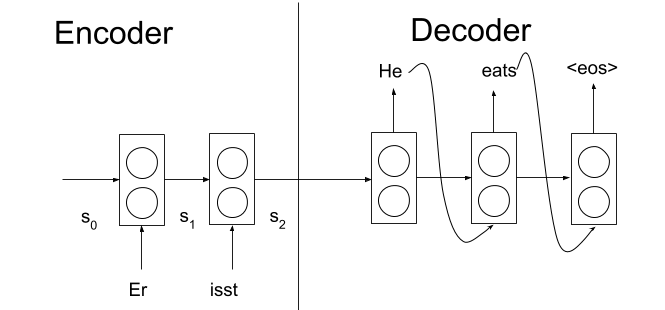
\includegraphics[width=\textwidth,height=10cm,keepaspectratio=true]
    {machine-translation-1.png}
    \caption{
        RNN network for machine translation \parencite{GerElmo}
    }
    \label{fig:machine-translation-1}
\end{figure}

Attention mechanism in neural networks is used to take two inputs and convert them into one common representation. This is done by configuring the level of attention that needs to be given to different parts of each input and combine them to form a single output. Most often the inputs will be matrices and the output will be a vector. Bidirectional RNNs can be used to convert both input and context information into matrices. The fixed output vector is then fed into a deep feed-forward neural network to predict a class. Attention mechanism with RNN gives state of the art results in many NLP applications such as Natural Language Inference \parencite{Parikh2016}, Machine Translation \parencite{bahdanau2014neural} and Document classification \parencite{Yang2016}.

\begin{figure}[H]
    \centering
    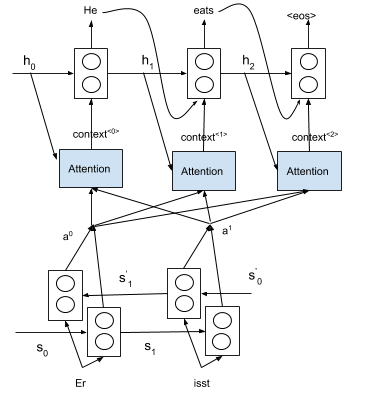
\includegraphics[width=\textwidth,height=10cm,keepaspectratio=true]
    {attention-networks-1.png}
    \caption{
        Attention network for machine translation \parencite{GerElmo}
    }
    \label{fig:attention-networks-1}
\end{figure}

\begin{figure}[H]
    \centering
    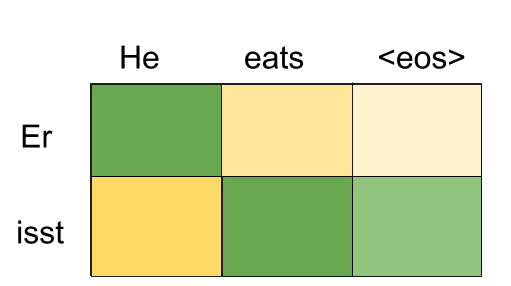
\includegraphics[width=\textwidth,height=10cm,keepaspectratio=true]
    {attention-matrix-1.png}
    \caption{
        Attention matrix 
    }
    \label{fig:attention-matrix-1}
\end{figure}


\subsection{Self-attention}


\parencite{Vaswani2017} - Attention is all you need

Each word or position representation is transformed into 3 vectors such as key $(k_t)$,  value $(v_t)$ and query $(q_t)$ with lesser dimensions $(d_k)$. This is done by using separate trainable parameters for word and position representation as well as for the above three entities. For example, the parameters for key transformation for both word and position representation are $W^{c}_K$ and $W^{p}_K$ respectively.

The attention of a word i to a word j in a sentence is then calculated as 
$ p(i\rightarrow{}j) \propto exp(\dfrac{q^{(c)}_i.k^{(c)}_j}{sqrt(d_k)}) $. In words, it is essentially a normalized dot product of respective query and key vectors. The weighted average of all values to form a average vector $\hat{v}_i = \sum_k p(i\rightarrow{}k)v_k$ represents the new value vector for word i which includes all the attention that it has on all the words in the sentence. 

The following set of equations reveal overall functionality of single attention head in mathematical terms. The query, key and value vectors are computed by respective weight parameters against the word representation. The output of this is a vector for each and every word. A matrix containing all the vectors concatenated represents the overall sentence and they are shown as $Q_p$, $K_p$, and $V_p$ respectively. The softmax function models the probability distribution of the dot product of query and key matrix. The dot product with value matrix computes the weighted average and it is transformed by $W^{(c)}_O$ matrix to align with other output dimensions.
\begin{align*}
q^{(c)}_t = W^{(c)}_Q c_t, k^{(c)}_t = W^{(c)}_K c_t, v^{(c)}_t = W^{(c)}_V c_t \\
SingleHead(C) = \left[softmax\left(\dfrac{Q_cK^T_c}{\sqrt{d_k}}\right) V_c\right] W^{(c)}_O \\
where\ Q_c = C{}W^{(c)}_Q; K_c = C{}W^{(c)}_K; V_c = C{}W^{(c)}_V  
\end{align*}

\begin{figure}[H]
    \centering
    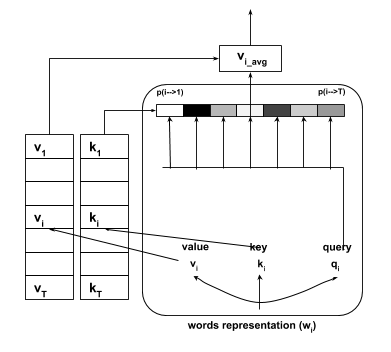
\includegraphics[width=\textwidth,height=6cm,keepaspectratio=true]
    {self-attention.png}
    \caption{
        Self-attention module
    }
    \label{fig:Self attention head}
\end{figure}

\begin{figure}[H]
    \centering
    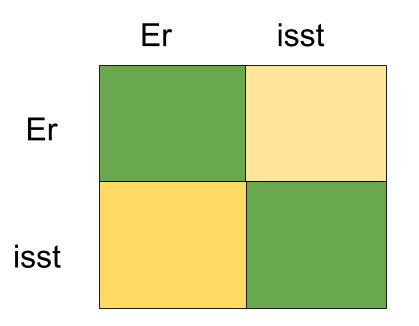
\includegraphics[width=\textwidth,height=10cm,keepaspectratio=true]
    {self-attention-matrix-3.png}
    \caption{
       Self-attention matrix 
    }
    \label{fig:self-attention-matrix-3}
\end{figure}


\subsection{CKY parsing}


Syntax structure can be modeled by Context-Free Grammars (CFG). Parsing attempts to extract the syntactic structure in the form of a tree from a sentence using the production rules specified in CFG.  A naive top-down search will take one of the starting non-terminals and proceeds to explore the non-terminals, all the way up to terminals and try to match the words. It explores many options that never connect to the actual sentence. Whereas a naive bottom-up search will start with words and try to match the non-terminal, all the way up to the starting terminal. It explores many options that can never lead to a full parse. The number of unsuccessful search depends on how much the grammar branches in each direction.

Cocke-Kasami-Younger (CKY) \parencite{YOUNGER1967189} is a bottom-up parsing and dynamic programming method that requires first normalizing the grammar. 

Two key issues that are dealt with by CKY parsing are computational complexity and ambiguity. The computational complexity is handled by using a chart that stores the previous recognition of production rules for word combination or sub-rule combinations and re-using it appropriately. 

\begin{figure}[H]
    \centering
    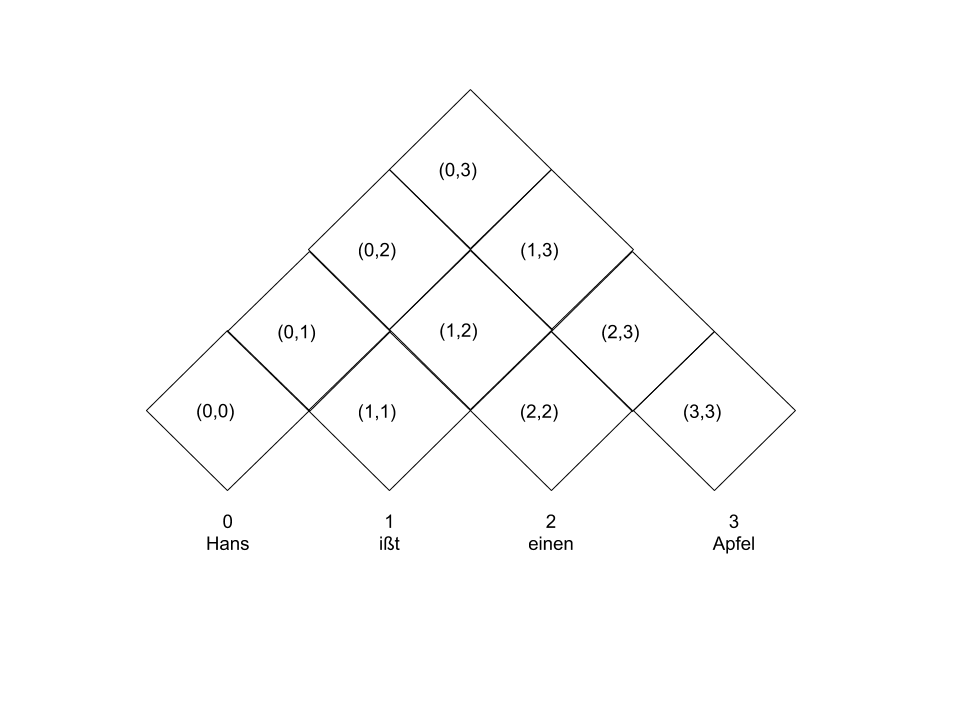
\includegraphics[width=\textwidth,height=8cm, keepaspectratio=true]
    {cky-parsing-chart-1.png}
    \caption{
        CKY chart
    }
    \label{fig:cky_parser_1}
\end{figure}

The ambiguity is dealt with by using Probabilistic Context-Free Grammar (PCFG). The probability values assigned to each production rule are used by parsing when they are assigned to sub-rule combinations and the importance of usage is computed. This importance is compared against other relevant production rules that could be applied and the best score is chosen.

The algorithm of CKY is explained briefly as follows: 
\begin{enumerate}
\item Convert the given grammar into  Chomsky Normal Form (CNF). This involves allowing only two kinds of right-hand sides in production rules such as either two non-terminals or one terminal. Any CFG can be written in CNF form.
\item Create a chart with the number of layers equivalent to the number of words in a sentence as shown in figure \ref{fig:cky_parser_1}. Each layer refers to the span of a sentence and so all possible combinations in a sentence will be explored
\item In the first layer, each word is dealt with. Replace the words with appropriate non-terminal(s) with the probability score
\item Look for unaries that can re-write non-terminals and if found then append those to appropriate cells in the chart. While adding recompute the new probability score by multiplying the appropriate production rule components (both left and right). This is continued until no possible replacement is available 
\item Look for the duplication for each non-terminal in each cell. If found then the one with the highest score is chosen and the rest are removed
\item When a layer with larger span is involved, use the results computed from a lower layer which is referring to smaller span. Consider all the possible cell pair combinations and for each cell pair, consider all the combinations of non-terminals from each cell. Say for e.g. for a span(0,2), the cell pairs {(0,0),(1,2)} and {(0,1),(2,2)} will be taken into account as shown in the figure \ref{fig:cky_parser_1}. Follow step 3 for the two non-terminals instead of words and also unary replacement steps. In each case compute the new probability score building from the previous cells. 
\item Keep on doing it until the span limit is covered. Take the non-terminal S, which is the starting terminal, with the highest score. If none found then the sentence cannot be parsed for a given grammar
\end{enumerate}

\begin{figure}[H]
    \centering
    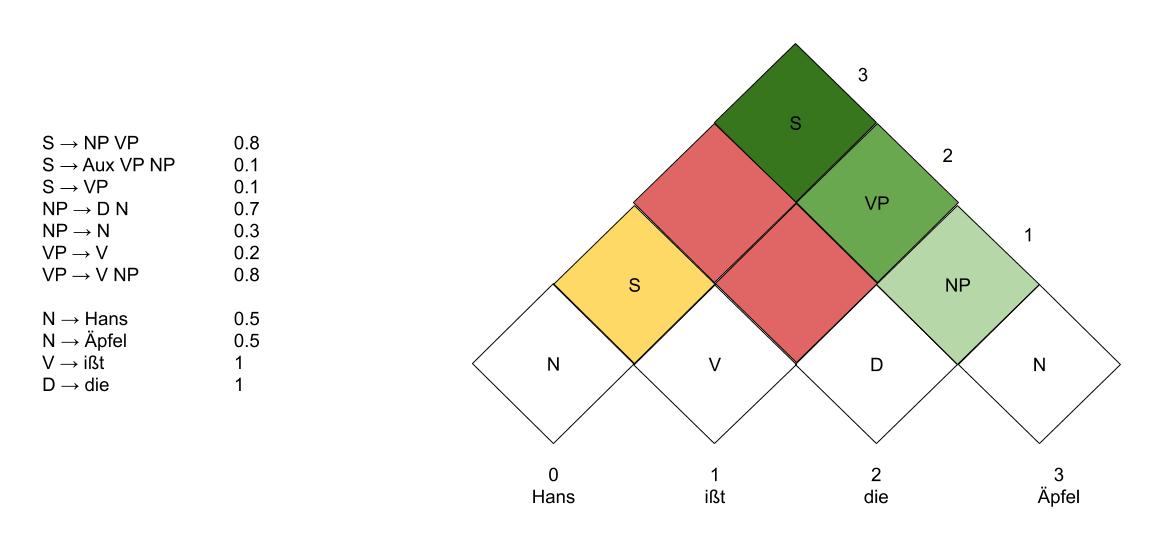
\includegraphics[width=\textwidth,height=8cm,keepaspectratio=true]
    {cky-parsing-chart-2.png}
    \caption{
        CKY parsing
    }
    \label{fig:cky_parser_2}
\end{figure}

In figure \ref{fig:cky_parser_2}, the sentence 'Hans isst einen Apfel' is parsed against PCFG grammar on the left side using CKY parsing and the tree produced is shown in green color in the chart. 'Hans' can be replaced with non-terminal N as in production rule N --> Hans and unary replacement NP --> N. The probability score 0.15 is computed by multiplying 0.3 and 0.5 that are taken from production rule and non-terminal N respectively. Certain combinations are not at all possible and they are referred to as red color in the chart. 


\pagebreak
\section{Approach}  

In this thesis work, deep learning techniques are used to develop constituent parser for german language. This section explains in detail the architecture used and the different components included in it. 

\subsection{Research Questions}

Through this work, the research questions that would be addressed are:
\begin{enumerate}
\item How well the self-attention based modules of neural networks are effective in capturing constituency grammar of german language? 
\item How efficient the model can be improved by using only the tree dataset? This means no other external data directly or indirectly will be utilized. 
\item How efficient the model can be improved using Transfer learning which involves pre-trained deep learning systems using external data such as German Wikipedia?
%\item What components of ELMo are useful for building an efficient model? ELMo uses a combination of three layers of its output data by computing a weighted sum of each layer. The research also involves figuring out which layer or what combination of layers output is pertinent to this particular task of developing a constituent parser.
\end{enumerate}

\subsection{Model}

The models are highly inspired from the works of Kitaev et al. \parencite*{Kitaev2019}, which involves an encoder-decoder architecture as shown in figure \ref{fig:broad_architecture}:

\begin{figure}[htpb]
    \centering
    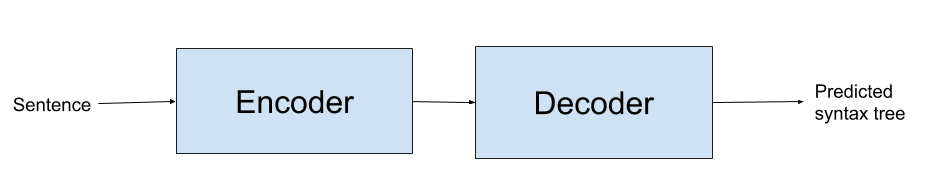
\includegraphics[width=\textwidth,height=8cm,keepaspectratio=true]
    {encoder-decoder.png}
    \caption{
        Broad Architecture
    }
    \label{fig:broad_architecture}
\end{figure}

The input to this system is a german sentence and the output is a predicted syntax tree of that particular sentence. The encoder takes in input sentence and does processing to convert it into a convenient, rich and versatile representation. This representation embodies information for each word with sub-word patterns as well as the context of the whole sentence. The encoded output is then fed into a decoder that outputs a syntax tree. The building of syntax tree is seen as a continuous iteration of merging of certain subsequent words or merges that already happened in hierarchy. The decoder method involves steps to figure out what combination of merges is the best to build a good syntax tree.

The training of a deep learning system involves a loss function to compare the prediction against golden output to allow fine-tuning of different components of the model using backward propagation of gradients of error. In this context, the predicted best possible syntax tree is compared against the golden tree and the parameters involved in the encoder section is updated accordingly to yield the best syntax tree next time. 

There are many ways by which the encoder and decoder components can be modeled. But in this approach, the encoder and decoder components are fixed and only the representation of sentences is varied to a certain degree. The encoder module is inspired from a state of art transformer neural network which predominantly uses self-attention modules, whereas the decoder module uses the CKY approach to build the syntax tree. Sentences are represented using character embeddings and different word embeddings. In addition to words, position information of words is also used separately. The system does not use any other pre-processed information such as Parts Of Speech (POS) obtained by an external tagger system as in old parsing methods.

\subsubsection{Encoder}

The purpose of the encoder, in this context, is to represent a sentence into a rich format that encompasses the sub-word patterns as well as the overall context of a sentence. This is achieved through multi-layered, multi-head attention modules backed up with feed-forward networks as shown in the figure \ref{fig:encoder_module}

\begin{figure}[htpb]
    \centering
    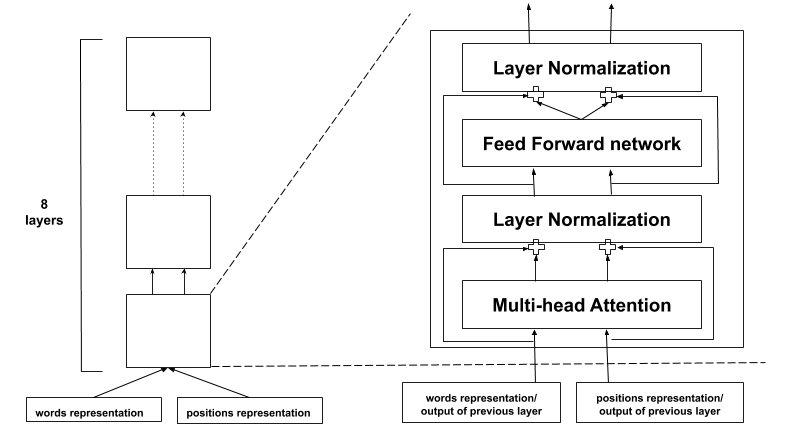
\includegraphics[width=\textwidth,height=15cm,keepaspectratio=true]
    {encoder.png}
    \caption{
        Encoder module
    }
    \label{fig:encoder_module}
\end{figure}

The input to this system is passed through $n_l$ identical layers made up of multi-head self-attention mechanism modules sequentially. The output of the first layer is passed as input to the second layer. At each layer, the representation of a sentence is expected to improve gradually. Multi-head attention uses $n_h$ single heads, whereas each one allows every word in a sentence to gather information from one word in the same sentence. This brings out a matrix of information regarding what words attend to or obtain information from what other words in a sentence. This is applied not only to words but also to positions separately. Kitaev et al. \parencite*{Kitaev2019} shown in their work that separating words and positions for building constituent parser improved the results by 0.5 \% F1 score. And also that, position attention contributes more than content attention by 18 \% F1 score. Hence the position attention is used separately. In their setup, value 8 for both $n_l$ and $n_h$ parameters gave better results. 

The output of Multi-head attention module is then passed to Layer Normalization by mixing with a residual component of input. The normalization of intermediate results along with objective function will help the gradient-based optimizer to arrive at the best values quickly. A feed-forward network at this juncture helps to look for patterns among the multiple attention representation of words in a sentence and also to map the intermediate result dimension space to be compatible with inputs and outputs of each layer.  

The dimensionality of representation, inputs, and outputs of each layer are the same. A total of 1024 neurons are used to represent and it is split half and used by word and position related functions respectively. 


The figure \ref{fig:single_attention_head} shows the outline of what happens inside a single attention head:

\begin{figure}[htpb]
    \centering
    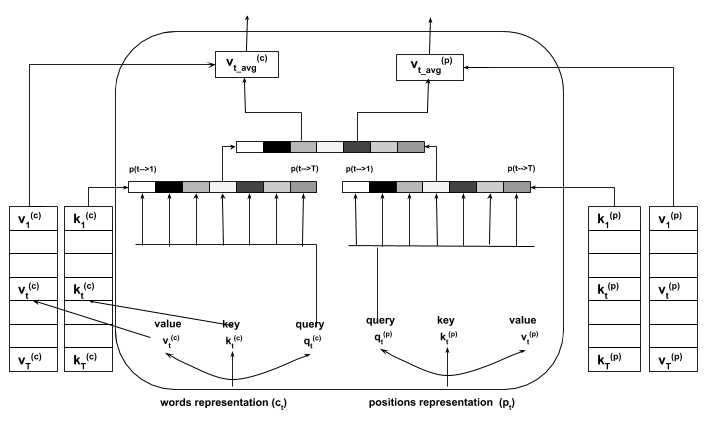
\includegraphics[width=\textwidth,height=10cm,keepaspectratio=true]
    {single-head-attention.png}
    \caption{
        Single attention head
    }
    \label{fig:single_attention_head}
\end{figure}


Each word or position representation is transformed into 3 vectors such as key $(k_t)$,  value $(v_t)$ and query $(q_t)$ with lesser dimensions $(d_k)$. This is done by using separate trainable parameters for word and position representation as well as for the above three entities. For example, the parameters for key transformation for both word and position representation are $W^{c}_K$ and $W^{p}_K$ respectively.

The attention of a word i to a word j in a sentence is then calculated as 
$ p(i\rightarrow{}j) \propto exp(\dfrac{q^{(c)}_i.k^{(c)}_j}{sqrt(d_k)}) $. In words, it is essentially a normalized dot product of respective query and key vectors. The weighted average of all values to form a average vector $\hat{v}_i = \sum_k p(i\rightarrow{}k)v_k$ represents the new value vector for word i which includes all the attention that it has on all the words in the sentence. 

The following set of equations reveal overall functionality of single attention head in mathematical terms. The query, key and value vectors are computed by respective weight parameters against the word representation. The output of this is a vector for each and every word. A matrix containing all the vectors concatenated represents the overall sentence and they are shown as $Q_p$, $K_p$, and $V_p$ respectively. The softmax function models the probability distribution of the dot product of query and key matrix. The dot product with value matrix computes the weighted average and it is transformed by $W^{(c)}_O$ matrix to align with other output dimensions.
\begin{align*}
q^{(c)}_t = W^{(c)}_Q c_t, k^{(c)}_t = W^{(c)}_K c_t, v^{(c)}_t = W^{(c)}_V c_t \\
SingleHead(C) = \left[softmax\left(\dfrac{Q_cK^T_c}{\sqrt{d_k}}\right) V_c\right] W^{(c)}_O \\
where\ Q_c = C{}W^{(c)}_Q; K_c = C{}W^{(c)}_K; V_c = C{}W^{(c)}_V  
\end{align*}

Similarly for position representation, the following equations convey single head functionality. Different set of trainable parameters are used to get the final output.
\begin{align*}
SingleHead(P) = \left[softmax\left(\dfrac{Q_pK^T_p}{\sqrt{d_k}}\right) V_p\right] W^{(p)}_O \\
where\ Q_p = P{}W^{(p)}_Q; K_p = P{}W^{(p)}_K; V_p = P{}W^{(p)}_V
\end{align*}

The output of single attention head is concatenated as shown in the figure \ref{fig:multi_head_attention_module}
\begin{figure}[htpb]
    \centering
    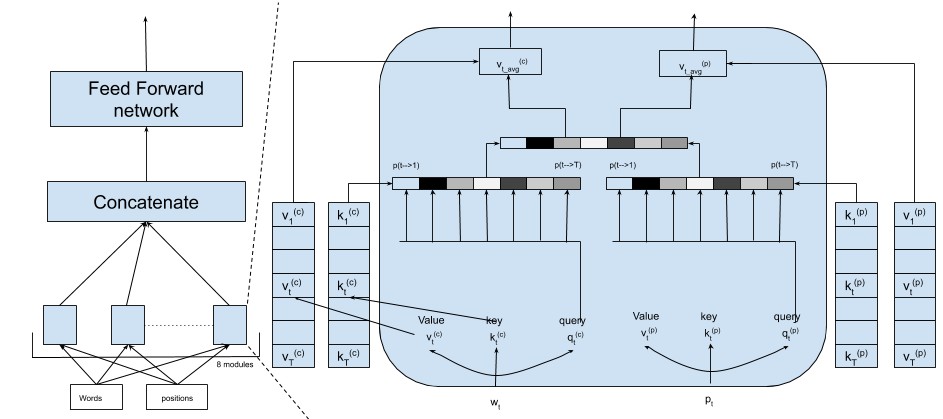
\includegraphics[width=\textwidth,height=10cm,keepaspectratio=true]
    {multi-head-attention.png}
    \caption{
        Mult-head attention module
    }
    \label{fig:multi_head_attention_module}
\end{figure}

The concatenated output fed through feed-forward to derive the patterns across multiple attentions in a sentence. These are then fed to Layer Normalization block as shown in figure \ref{fig:encoder_module}.

\subsubsection{Decoder}
The decoder of this parser is inspired by the works of Stern et al. \parencite{Stern2017} and Gaddy et al. \parencite{Gaddy2018}. The output of encoder is a matrix wherein each row vector of size 1024 neurons represents a word in a sentence. The quantification of how good a combination i and j is considered as a constituent with label l is computed by scoring modules. The combination of two entities i and j is represented by a vector  $v = [\overrightarrow{y}_j - \overrightarrow{y}_i; \overleftarrow{y}_{j+1} - \overleftarrow{y}_{i+1}]$. The vector of size 1024 for a word or entity is divided into two vectors of equal size to be used as a representative for the left or right part of a constituent. The computed vector v for entities i and j  is transformed non-linearly with normalization into a space of size equal to the number of labels. The label information is obtained by going through all the training samples and used to predict the label as well as the scores associated with it. 

\begin{align*}
s(i,j,l) = M_2relu(LayerNorm(M_1v + c_1)) + c_2
\end{align*}

\begin{figure}[H]
    \centering
    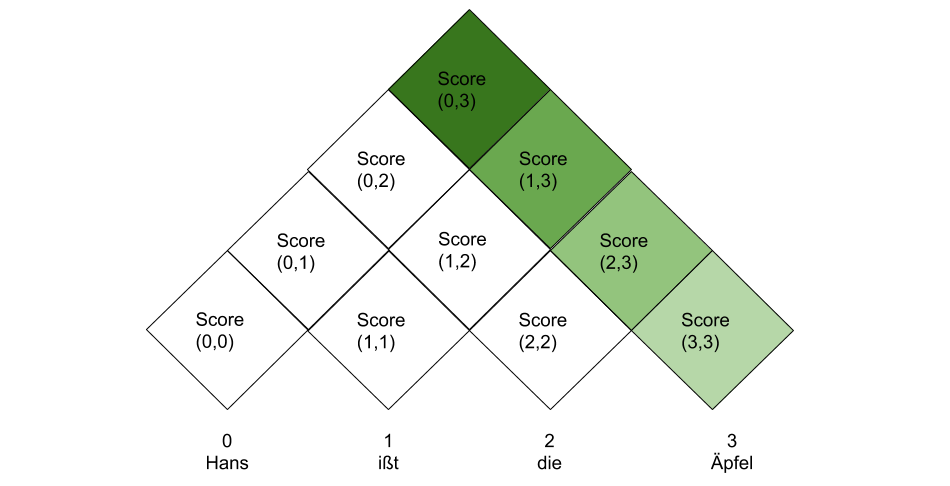
\includegraphics[width=\textwidth,height=10cm,keepaspectratio=true]
    {cky-parsing-chart-3.png}
    \caption{
        CKY parsing with scores
    }
    \label{fig:CKY}
\end{figure}

The decoder uses CKY parsing to compute scores for all the combinations and also computes the best overall tree $\hat{T}$ as the sum of all best subtrees. There are no defined PCFG grammar and its components associated with it. Every combination is a production rule, every label in a training set is a non-terminal, every word is a terminal and all non-terminals are starting terminals. The score for a combination is considered as probability value of a production rule. The best score for a combination $s_{best}$ is obtained by the sum of its label score and best split that can divide the combination recursively. For consecutive entities, it is based only on the label score.

\begin{align*}
s(T) = \sum_{(i,j,l) \epsilon T}s(i,j,l) \\
\hat{T} = \underset{T}{\mathrm{argmax}}\ s(T) \\
s_{best}(i,i+1) = \underset{l}{max}\ s(i,i+1,l) \\
s_{best}(i,j) = \underset{l}{max}\ s(i,j,l) + \underset{k}{max}\ {\left[s_{best}(i,k) + s_{best}(k,j)\right]}
\end{align*}

\subsubsection{Training}

A max-margin based objective function is used to ensure that training of constituent parser results in the right parser tree.

\begin{align*}
max\left(0, \underset{T\neq{T^*}}{max}\left[s(T) + \Delta(T,T^*)\right] - s(T^*)\right)
\end{align*}

Here $T^*$ is the golden tree and s(T) refers to all the possible trees except the golden tree. $\Delta$ used is a Hamming loss computed for golden and predicted tree. In this system, for every comparison of subtree with label failing between golden and predicted tree, a value 1 is summed.

With this training approach, the score of a golden tree will be maintained higher than any other tree by a margin of $\Delta$.  

\begin{align*}
s(T^*)\ \geq s(T) + \Delta (T,T^*) \\
\end{align*}

Here, the parsing ability of the system is not only learned but also the PCFG grammar of German. While trying to maintain the score for a golden tree to be high, the scores for combinations are fine-tuned which is analogous to the probability values of that production rule.

\subsection{Experiments}

The experiments are different for each pursuit of research questions. But the findings of one research are used in the subsequent researches. 

\subsubsection{Research Question 1}
The first research question address how effectively the self-attention module can be utilized to maximize the optimal building of constituent parser. The following points cover the idea of experiments that will be conducted for this scenario:
\begin{enumerate}
\item The first parameter that controls the self-attention module is the number of self-attention heads $(n_h)$. This helps the system to let the words to gather information from multiple locations in the same sentence. 
\item The next parameter which influences the output is the number of identical layers $(n_l)$ that are stacked above each other. It helps the system to draw generalized or abstract or deep patterns from the primitive low-level patterns already computed. 
\item The internal dimension parameter for key, value and query attributes. This is used in conjunction with several self-attention heads. In this approach, this is assigned with a fixed value 64 and the first parameter is changed. This particular value is taken from the research carried out by Kitaev et al. \parencite*{Kitaev2019}
\end{enumerate}

The assumption is that the more the value the better the result will be. But after some point, the rate of returns will be diminishing. A range of values are assigned to both the parameters and experiments will be conducted. The result metric will be computed and tabulated as shown below:

\begin{table}[h!]
  \begin{center}
    \begin{tabular}{c|c|c|c|c|c|c} 
      $n_l/n_h$ & $1$ & $3$ & $5$ & $8$ & $10$\\
      \hline
      1 & & & & & & \\
      \hline
      3 & & & & & \\
      \hline
      5 & & & & & \\
      \hline
      8 & & & & & \\
      \hline
      10 & & & & & \\
    \end{tabular}
    \caption{Parameters range table for Research question 1}
    \label{tab:research_question1_table1}

  \end{center}
\end{table}

Ideally, all the variables should be changed and the result metric should be computed and tabulated. The pair of $(n_l,n_h)$ values for which the resultant metric value is high, will be chosen as an ideal combination. But given the limitation on computation power and also the time, instead of choosing a classical Grid search which covers all the 100 combinations, a random set of pairs will be chosen. In addition to that, Kitaev et al. from their research, chose value to be 8 after hyper tuning for both $n_l$ and $n_h$ respectively. Given these conditions, fewer experiments will be conducted to find out the ideal pair.

\subsubsection{Research Question 2}

The second research question is intended to explore building the best possible constituent parser using only training data. In the previous case, the self-attention model is analyzed by trying out different values for the number of identical layers and the number of attention heads. 

The input representation is expressed using an embedding matrix. Each component of input is represented using a row or column vector. Upon passing an index, the respective vector is retrieved. For example, in the case of words, each word is given a unique index $i$ and represented by a row vector $w_i$ with $d$ dimension as follows:

\begin{center}
$\begin{bmatrix}
    w_{11}       & w_{12} & w_{13} & \dots & w_{1d} \\
    w_{21}       & w_{22} & w_{23} & \dots & w_{2d} \\
    \hdotsfor{5} \\
    w_{n1}       & w_{n2} & w_{n3} & \dots & w_{nd}
\end{bmatrix}
$

\end{center}

Similar is the case for position representation as well. In this experiment, the representation of input is trained along with other parameters. So, with every batch, it is expected to learn effectively. The various representation of input to the system with only training data is explored as follows:

\begin{enumerate}
\item Character embeddings matrix represents each character used in the training set with a vector. To be on the safer side, a maximum range for the no.of characters is selected by analyzing the training dataset. The representation for each word will be constructed by using a bi-directional LSTM based RNN network. For each character in the word, the RNN is unrolled in sequence and the two last output vectors will be obtained by traversing left to right and vice-versa. Those two final vectors are merged to form the final vector to represent the word.
\item Instead of characters, an embedding matrix is constructed where each vector represents a word directly. For all the words that do not exist, a unique vector labeled as <UNK> will be used. 
\item The third alternative is using both character and word embeddings matrix. The dimension of both the matrix will be fixed and the resultant vectors from those matrices are added together to represent a word. 
\end{enumerate}

With character embeddings, the words which are not present in the training dataset will still be expected to be assigned with a reasonable appropriate vector. The character embeddings are expected to learn sub-word patterns and use them when constructing unknown words. For each word, the vector is constructed on the fly, whereas with word embeddings, the vectors are fixed. The word embeddings as stated by Mikolov et al. \parencite{mikolov2013linguistic} is expected to learn similarities. But using <UNK> vector will not be as effective as the former strategy. By combining both character and word embeddings, the benefits of both are expected to be utilized. 
\subsubsection{Research Question 3}

The third research question addresses the usage of Embeddings from Language Models (ELMo). In addition to that, what components or combination of them helps build an efficient parser. ELMo embeddings are constructed using a multi-layer, character convolution-based, bi-directional LSTM modules by training with a very large dataset at least over a billion tokens. The representations are deep and have provided state of the art results in various application systems. As stated in the section ???, it outputs 3 layers and the following section shows the experiments to be conducted with ELMo:


\begin{enumerate}
\item The first layer of ELMo does not involve any context and it is constructed by the concatenation of character embeddings with a feed-forward network. This will be used as a base model for these experiments and it is expected to give least favorable result. This is much closer to using only character embeddings as specified in the previous research. But these are the result of training from external, rich resources such as Wikipedia. The expectation of a relatively better result is still valid.
\item The data of second layer of ELMo is the output of first bi-directional language model module. It also embodies the syntactic relations of the different words in a sentence. As constituent parsing also is a syntactic relation extraction, this layer output will be very useful. 
\item The data of third layer of ELMo is the output of second bi-directional language model module. It embodies the deep, contextual relationship of words in a sentence. It will be interesting to see how does this layer influences the parser as compared to the second layer.   
\item Using all the combinations of layers by training scalar weights which will be used as a weighted average of outputs of all the layers. This will be specific to the constituent parsing task and at the same time expected to use the benefits of all three layers. 
\end{enumerate}

All the above experiments will reveal how best ELMo can be used in building an effective constituent parser. 


\pagebreak
\section{Evaluation}

This section covers how the system will be evaluated as a constituent parser. In this master thesis, the focus is mainly on improving the quality of the system and the speed of the system can be improved by using good hardware. Dataset and the metric are the two most important factors play a major role in achieving the evaluation. 
\subsection{Dataset}

The TüBa-D/Z treebank \parencite{TubingenTreebank} released by the University of Tübingen is used to train constituent parser. The dataset consists of 104,787 sentences that are divided randomly into training, development, and test dataset of size 84,787, 10,000, and 10,000 respectively. The development dataset is used to fine-tune the hyper-parameters of the model after getting trained with the training dataset. The test dataset is used to measure the quality of constituent parser at the end. 

\subsection{Metrics}

To measure the quality of a constituent parser, the predicted syntax tree should be compared with the respective golden tree. A comparison of two trees involves comparing all their subtrees for a match. With the extraction of subtrees from both gold and predicted trees, there will be two sets of trees to be compared against.

The following table shows the confusion matrix for a constituent parser:

\begin{table}[h!]
  \begin{center}
    \label{tab:table1}
    \begin{tabular}{c|c|c|c}
      &  \multicolumn{3}{c}{Predicted Tree}\\
	  \hline
      \multirow{3}{*}{Golden Tree} & & \textbf{Negative} & \textbf{Positive} \\
      & \textbf{Negative} & True Negative & False Positive \\
      & \textbf{Positive} & False Negative & True Positive\\
    \end{tabular}
    \caption{Confusion matrix}
  \end{center}
\end{table}

The terms described in the above table are generic. But it involves some differences in the context of tree comparison, which is explained as follows:
\begin{itemize}
\item True Positives are set of subtrees which are present in both golden and predicted tree. That is the parser system predicted correctly the constituent in a sentence.
\item True Negatives are set of subtrees which are not in both golden trees and predicted tree. In an information retrieval system, it makes sense, since the system can correctly leave the unrelated documents. But in this case, it will always be zero.
\item False Positives are set of subtrees that are there in predicted tree but not in the golden tree. This means that the parser wrongly selected a range of entities as a constituent. 
\item False Negatives are set of subtrees that are there in golden tree but not in predicted. This means that parser failed to select a range of entities as a constituent which it should have. 
\end{itemize}

The quality of the system can be measured by metrics such as Precision, Recall, and F1 measure. Each one can be computed using the formula as follows:
\begin{align*}
Precision = \frac{True\ Positive} {True\ Positive + False\ Positive}
\end{align*}

\begin{align*}
Recall = \frac{True\ Positive} {True\ Positive + False\ Negative}
\end{align*}

\begin{align*}
F1 = \frac{2* Precision * Recall} {Precision + Recall}
\end{align*}

Precision focuses completely on the output of the system which is being measured. It is possible to develop a parser that finds only one right constituent. This will give a 100\% precision but a terrible constituent parser. At the same time, recall focuses completely based on the output of golden tree. It is possible to develop a parser to list all possible combinations and regard them as constituents. This will end up giving a 100\% recall.

F1 measure takes in a balanced approach by involving both precision and recall. It is preferred since it includes both false positive and false negatives. The F1 score is computed for each predicted output tree and an average is computed for all the trees in a batch. 


\pagebreak
\section{Implementation}

This section covers the implementation details for building a constituent parser. All the programs required to build the parser using neural networks are written in python (3.7.4) \footnote{https://www.python.org/downloads/release/python-374/}. The model built is relatively complex and involves a lot of parameters. The training of these parameters approximately took one day using GeForce GTX 1050 Ti GPU. And so, it is important to have a good GPU configuration to run and train the model effectively. 
\subsection{Dependency management}

The main dependencies of the program are listed below:
\begin{itemize}
\item CUDA \footnote{https://developer.nvidia.com/cuda-zone}, a parallel computing platform and programming model developed by NVIDIA for general computing on GPU
\item Pytorch (1.3.1) \footnote{https://pytorch.org/}, an open-source machine learning framework, written in python, has immense support for tensor computation with GPU acceleration, automatic differentiation, and a huge set of library function to ease development experience
\item Cython (0.29.14) \footnote{https://cython.org/}, optimized static compiler, helps python code to call back and forth from and to C or C++ code natively. The decoder part of this project is written in Cython to improve parallelism and speed. All the possible combination of constituent formation has to be analyzed for forming the best-predicted tree using CKY method.
\item AllenNLP (0.9.0) \footnote{https://allennlp.org/}, an open-source NLP research library, built on PyTorch. ELMo module, an important component of this project, is taken from AllenNLP libraries.  
\end{itemize}

\subsection{Source code}

The source code\footnote{https://github.com/Kandy16/self-attentive-parser} is highly inspired and derived from the published GitHub code \footnote{https://github.com/nikitakit/self-attentive-parser} of Kitaev et al. \parencite*{Kitaev2019}. There have been modifications made on Encoder, and ELMo modules to suit the project needs. Their work did not focus on using ELMo modules for the German dataset. Also, the code is upgraded to use the latest version of dependencies, API support for an extension. The code includes a CLI support for configuring all the parameters.

%Cython implementation

May et al. \parencite*{GerElmo} worked on building an ELMo based word representation for German language using German Wikipedia. The source and also the pre-trained data are shared in a GitHub project \footnote{https://github.com/t-systems-on-site-services-gmbh/german-elmo-model}. Their implementation followed exactly the works of E.Peters et al. \parencite{peters2018deep} and also the model serialization format and accessibility followed the same standards of AllenNLP format.

For parallelism to work smoothly, the arbitrary sentences and words should be of same length to have same size matrix. Instead of fixing the size for all the sentences, a quick pass is made on one particular batch and the maximum number of words in a sentence and also the maximum number of characters in a word is obtained. Using this information the matrices are constructed and parallelism is achieved. In this process, to let the system explicitly know the start and end of sentence or word, unique tokens are added at the beginning and end. The works of  Kitaev et al. \parencite*{Kitaev2019} showed a considerable improvement in the quality of parser after adding these tokens.

\subsection{Deployment}

The model is stored in PyTorch specific serialization format. The model is trained on training dataset through batches. All these inputs are parameterized and depending on the choice of the number of epoch and number of batches, the training dataset is divided into respective batch sizes. By default, at regular intervals, four times during one epoch, the performance of the model is compared against the development dataset and when the F1 score is better than the best scored in past, the model is replaced. The training of the model can be stopped by specifying the number of epoch or when the model did not give better results consecutively for the configured number of times. All these configurations can be changed as per convenience before the start. 

A docker\footnote{https://www.docker.com/} container image is a lightweight, standalone, executable package of software that includes everything needed to run an application. This makes the distribution of dependencies for a system much efficient and can avoid virtual hardware in most of the cases. A docker interface is created for both source code, and model, which can be executed on any machine as long as the CUDA is compatible. 



%Recurrent neural networks will be used in this master thesis extensively since they perform well with sequential data. TensorFlow\footnote{https://www.tensorflow.org/} is a python library for building intensive numerical computation applications and deploy them in multiple platforms such as CPU and GPU. TensorFlow has built-in libraries to develop different neural network architectures. Wikipedia consists of a lot of articles; each article consists of a lot of sentences. Each sentence will be fed as input to the neural network.
%---------------
%An advanced RNN architecture takes in either one or two inputs such as sentence in Wikipedia and context information. The context can be empty. The system processes the input and produces a binary output representing true or fake news. The outputs would contain a probability distribution of how likely it is true or fake news.

%The inputs, in general, will be pre-processed to extract tokens, remove common words such as articles, prepositions and perform lemmatization which is converting the words to its root form. Low dimensional and dense word embeddings will be used to represent the inputs instead of one-hot vectors. Already available word embeddings such as Word2vec \parencite{Mikolov2013} and GloVe\footnote{https://nlp.stanford.edu/projects/glove/} will be used to represent the inputs.

%The dataset will be split and used for training, validation, and testing of the system. A general rule of thumb is to divide the dataset into 60-20-20 for training, validation, and testing respectively. But if the datasets are in order of millions then it is good enough to have approximately 10000 entries each for validation and testing. The validation dataset is used to try out different hyper-parameter configurations and select the optimal values for each. The hyper-parameters of the advanced neural network system that will be configured are number of layers, learning parameter, batch size, activation functions and epoch number(number of times the training dataset should be iterated).

% Background Knowledge: Wikidata or BabelNet (knowledge graphs), http://babelfy.org/ for entity resolution

%The proposed methods involve modeling the content of Wikipedia in different ways such that the system can understand it better. These procedures are completely automatic in building the training examples and none of the features will be manually crafted. The different configurations of the system along with unique methods in constructing the training data is expected to understand Wikipedia better and the fake news detection can be carried out in a platform-agnostic manner. 

% ----------------------------------------------------------------------------



\pagebreak
\section{Analysis}

This section reveals the results achieved for every research question and also analyses the possible reasons for the outcomes.

\subsection{Research Question 1}

In this section, how well the self-attention modules are effective in capturing constituency grammar of German language is analyzed. The values for number of layers $(n_l)$ and number of attention heads $(n_h)$ are changed and for each combination, the model is trained and checked against development dataset four times in one epoch. Once when the development F1 score reached saturation or started decreasing over some time then the program is stopped. Once when the training is completed, the model is made to predict the sentences in the test dataset and compared against its actual output tree. 

\subsubsection{Optimal values for $n_l$ and $n_h$}

Since the number of possible combinations of different values would lead to 100 and each training takes more than a day, training for all the combinations will be time-consuming. The methodology used is a coarse-fine search to find the right combination. Initially, the combination of values is widespread covering the whole spectrum and the models are trained. Depending upon the results, the window of search is restricted but the granularity of search is increased. The following table shows the coarse search of parameter values and their results with the trained model:

\begin{table}[h!]
  \begin{center}
    \label{tab:coarse_search_for_layers_heads}
    \def\arraystretch{1.5}%  1 is the default, change whatever you need
    \begin{tabular}{c|c|c|c}
      \textbf{$n_l$} & \textbf{$n_h$} & Dev F1 (\%) & Test F1 (\%) \\
      \hline
      1 & 1 & 90.05 & 89.98\\
      3 & 3 & \textbf{92.47} & \textbf{92.44}\\
      5 & 5 & \textbf{93.83} & \textbf{92.77}\\
      8 & 8 & 87.95 & 87.82\\
      10 & 10 & 86.27 & 86.30\\
    \end{tabular}
    \caption{Performance of models with different $n_l$ and $n_h$ values}
  \end{center}
\end{table}

A total of five searches and each one covering a new value for $n_l$ between 1 and 10 and they are equally spaced. From the table above, it is evident that the performance of parser was improving until 5 and then it started declining. From the results, when the values are increased further, it is reasonable to assume that the performance of parser will decline even more. 

From the table, it is clear that $n_l$ values as 3 and 5 gave good results. A fine search is carried for values 3 to 5 and the results are published in the following table:

\begin{table}[h!]
  \begin{center}
  \def\arraystretch{1.5}%  1 is the default, change whatever you need

    \label{tab:fine_search_for_layers_heads}
    \begin{tabular}{c|c|c|c}
      \textbf{$n_l$} & \textbf{$n_h$} & Dev F1 (\%) & Test F1 (\%) \\
      \hline
      \multirow{5}{*}{3} & 1 & 91.80 & 91.78\\
	  & 3 & 92.47 & 92.44\\
	  & 5 & \textbf{93.60} & \textbf{93.68}\\
	  & 8 & 91.98 & 92.00\\
	  & 10 & 92.84 & 92.86\\
	  \hline
      \multirow{5}{*}{5} & 1 & 92.75 & 92.78\\
	  & 3 & 92.37 & 92.37\\
	  & 5 & 92.83 & 92.77\\
	  & 8 & 92.48 & 92.50\\
	  & 10 & 92.27 & 92.24\\
    \end{tabular}
    \caption{Performance of models with $n_l$ values as 3 and 5}
  \end{center}
\end{table}

Instead of doing a fine search, all the values are tried including even values for $n_h$. The value 4 is also tried for $n_l$ which is not tabulated. From the table, it is evident that the value 3 for $n_l$ and 5 for $n_h$ gives a maximum test F1 score of 93.68\%. This combination is tested multiple times and the results are quite consistent. This combination will be used for further researches. 

\subsubsection{Self-attention module - how well it captures context? }

From table \ref{tab:coarse_search_for_layers_heads}, it is surprising to know that one layer and one attention head captures the essential pattern that it can achieve almost 90\% test accuracy. This shows that self-attention heads are much effective in building a constituent parser. It captures the context of sentence much effectively which is used by high-level layers including the scoring module.

The self-attention matrix reveals how much each of the words is influenced by other words in the same sentence. The larger the value, the greater the influence that word has. The values need not sum up to 1, but for an understanding purpose, this relatively exposes how does the influence is distributed. 

The figure \ref{fig:self-attention-head-matrix} shows self-attention matrix of a sentence with four words 'Hilfe für kriegstraumatisier-te Frauen'. In this, the word 'Hilfe' has a relatively higher influence on the whole sentence. Each value is color-coded; the higher the value then the brighter it is.

\begin{figure}[H]
    \centering
    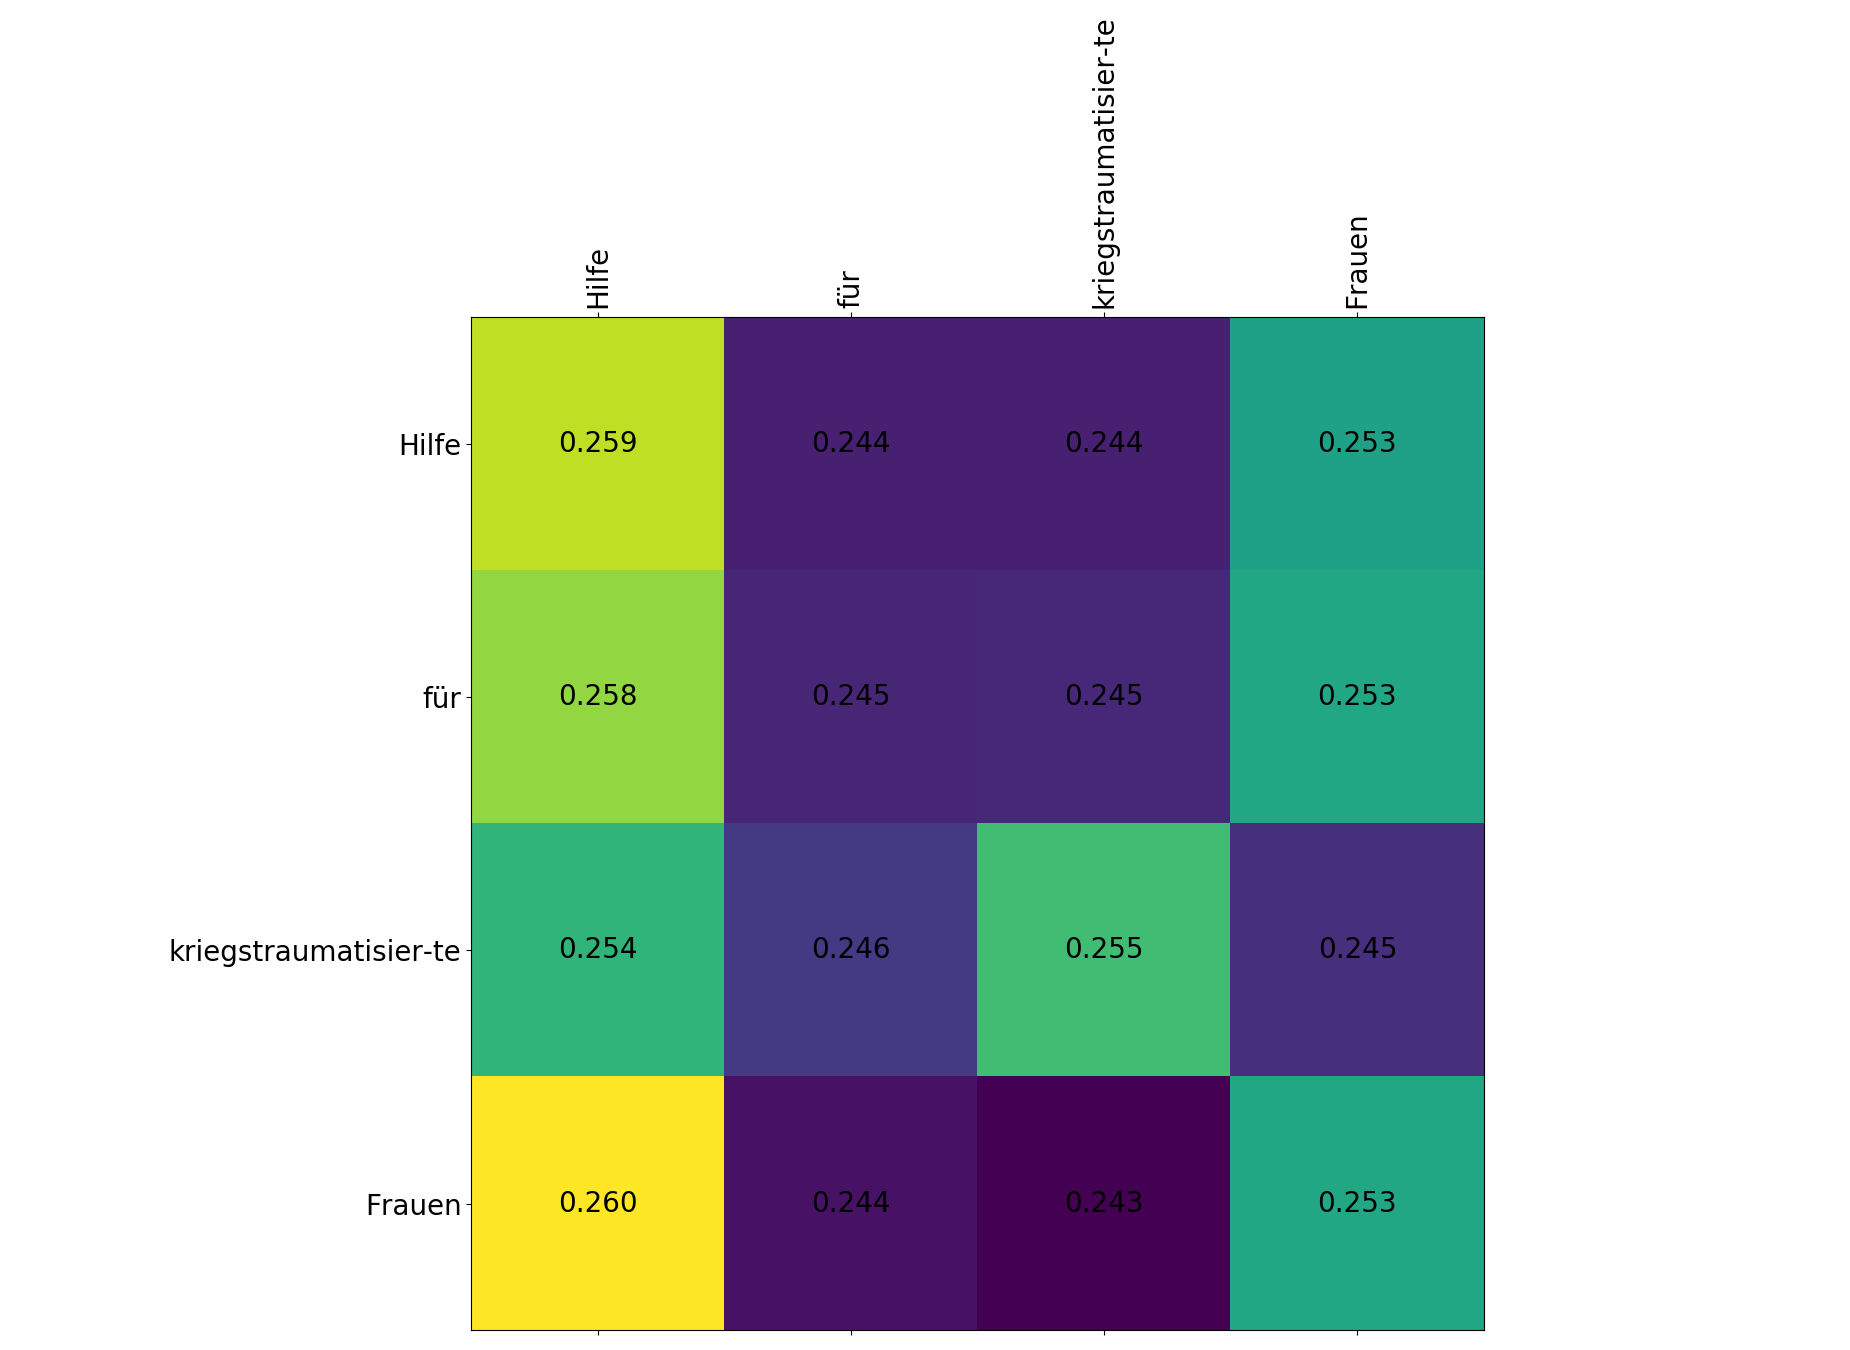
\includegraphics[width=\textwidth,height=10cm,keepaspectratio=true]
    {attention-head-matrix.png}
    \caption{
        Self-attention head matrix
    }
    \label{fig:self-attention-head-matrix}
\end{figure}

From the above experiments, $n_l$ and $n_h$ values as 3 and 5 gave best results. A total of 15 attention heads is being used in the model. Out of which, 5 attention heads act on input directly and independent of each other. The output of it is combined and passed to 5 attention heads and so on.  So, in the second layer of attention heads, the influence of influences of first 5 attention heads is computed or learned instead of the words. This will help the system to learn abstract patterns or a higher level of understanding of context. The final layer improves the understanding of context along the same lines.

The figures \ref{fig:self-attention-matrix-small-sentence} and \ref{fig:self-attention-matrix-large-sentence} show the self-attention matrix of 15 heads arranged in 3 layers. From the analysis of it with multiple sentences, the following are the findings:

\begin{itemize}
\item Every self-attention module in the same layer captures different influences. There are hardly any strict similarities. There is a slight variation from other modules. This means that the system can capture different influences and segregate them efficiently through training. This representation will be quite efficient as it is very clear for higher layers to act upon 
\item  The influence is strong on fewer entities in the first layer. In the sentence 'Der Streit ist längst nicht entschieden', it is evident that the first layer contains distinct influences, the words 'der', 'Streit', 'ist', and 'längst' gets influenced predominantly by one word. Whereas in the subsequent layers, the influence is shared among other entities to a certain degree. This shows the abstraction or higher-level understanding of the influences of entities

\item The behaviors are the same for longer sentences. In the figure \ref{fig:self-attention-matrix-large-sentence}, the sentence has 20 words and the same pattern is observed. Each self-attention model observes different influences and as the layers go up, the distinction of influences is distributed across all entities
\end{itemize}

\begin{figure}[H]
    \centering
    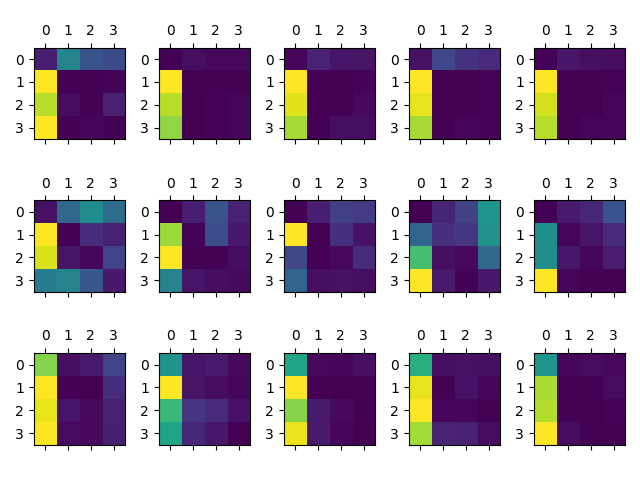
\includegraphics[width=\textwidth,height=10cm,keepaspectratio=true]
    {self-attention-matrix-1.png}
    \caption{
        Self-attention matrix of small sentence
    }
    \label{fig:self-attention-matrix-small-sentence}
\end{figure}

\begin{figure}[H]
    \centering
    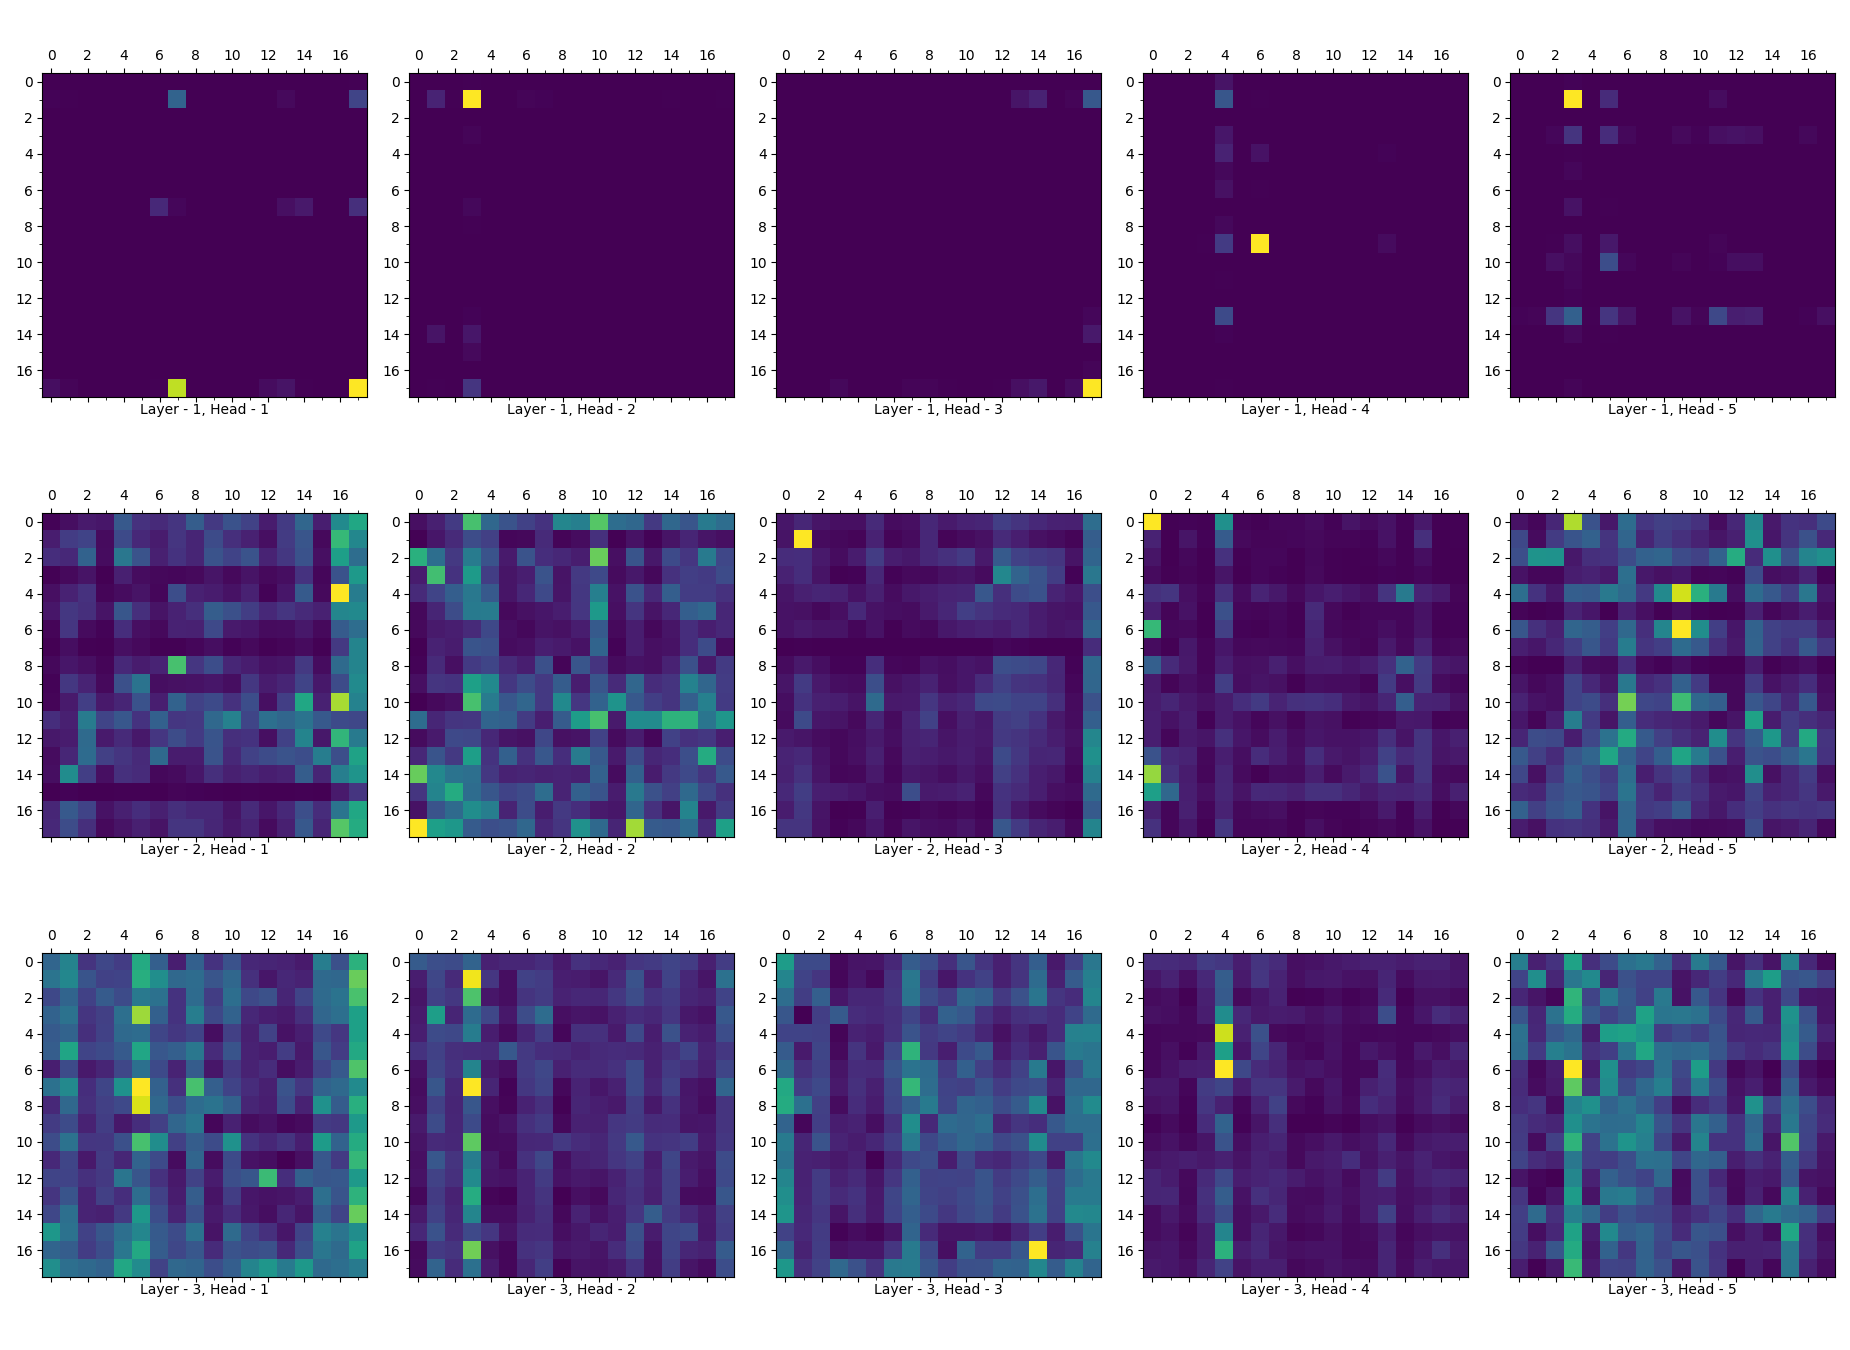
\includegraphics[width=\textwidth,height=10cm,keepaspectratio=true]
    {self-attention-matrix-2.png}
    \caption{
        Self-attention matrix of long sentence
    }
    \label{fig:self-attention-matrix-large-sentence}
\end{figure}

%\subsubsection{Tree analysis - what it captures and what it does not ?}

\subsection{Research Question 2}

In the previous section, the role of self-attention modules is analyzed. In this how effective a model can be implemented for constituent parser using only the dataset which is the sentence and the labeled syntax trees. The representation of the sentence is subjected to changes and the model is trained separately. 

At first, the input is represented using character embeddings whereas each character is referred by a vector and the word is summation of all the vectors that represent each character in the word. Secondly for each word in a sentence is represented a unique vector. In the third experiment, both character embeddings and word embeddings are used together. They are added up to refer to a word in the sentence. The table below reveals the model development and test F1 score as follows:

\begin{table}[h!]
  \begin{center}
    \label{tab:different_embeddings_model}
    \def\arraystretch{1.5}%  1 is the default, change whatever you need
    \begin{tabular}{c|c|c}
      Embeddings based models & Dev F1 (\%) & Test F1 (\%) \\
      \hline
      Character embeddings & \textbf{93.60} & \textbf{93.68}\\
      Word embeddings  & 91.22 & 91.16\\
      Character + Word embeddings & \textbf{94.17} & \textbf{94.10}\\
    \end{tabular}
    \caption{Performance of different emdeddings based models }
  \end{center}
\end{table}


From the table, it is quite evident that embeddings play an important role in improving the accuracy and some important understanding are as follows:
\begin{itemize}
\item Character embeddings are better than word embeddings. By using the former, the F1 score is improved by 2.5\% on the test dataset. %This validates the consensus that character embeddings perform better in most NLP applications than using word embeddings. (Try to add citations???)
\item Involving both character and word embeddings to represent input performs better than using them individually. A performance improvement of 0.42\% F1 score on test dataset is achieved. Although it is very marginal, this level of improvement beyond 90\% is important
\item It is observed that 4.8\% of words in test dataset do not appear in training dataset. In case of word embeddings all unknown words are represented using a unique <UNK> vector whereas in character embeddings all unknown words can be represented with different vectors since all characters are covered in training dataset itself
\item Also character embeddings are capable of learning sub-word patterns since the granularity of representation is much stronger than word embeddings. To add credibility to it, it is made sure that words that appear only in test dataset but not in training dataset are replaced with <UNK> token and so even in character embeddings there will be only one unique vector to represent all unknown words. Even with this arrangement, the character embeddings performed better in the same way than word embeddings. This adds validity that character embeddings representation offers an opportunity for the system to learn better. 
\end{itemize}

%\subsubsection{Distance analysis - meaning}
%pickup some words - compute the distance representation

%\subsubsection{Tree analysis - what it captures and what it does not ?}

\pagebreak
\subsection{Research Question 3}
So far the best possible model for a constituent parser that could be developed using only the training dataset is tried out. In this section, with the use of a pre-trained model using external data, how efficient a constituent parser can be built is analyzed.

For this, ELMo modules which are built from German Wikipedia with more than 1 billion tokens are used to represent the input instead of character or word embeddings. This ELMo uses 2 layers of bi-directional LSTM on character convoluted input. The input layer which is the first layer is composed of a function of character embeddings network. The second layer is the first bi-directional LSTM network output and the third layer is built on top of the previous. The following table shows the performance of constituent parsing when these layer inputs are used separately and combined:

\begin{table}[h!]
  \begin{center}
    \label{tab:different-elmo-models}
    \def\arraystretch{1.5}%  1 is the default, change whatever you need
    \begin{tabular}{c|c|c}
      ELMo based models & Dev F1 (\%) & Test F1 (\%) \\
      \hline
	  First layer & 92.79 & 92.86\\
      Second layer  & \textbf{95.43} & \textbf{95.49}\\
      Third layer & 94.69 & 94.79\\
      Combination of all layers & \textbf{95.76} & \textbf{95.87}\\     
    \end{tabular}
    \caption{Performance of different ELMo based models}
  \end{center}
\end{table}

From the table, it is clear that layered outputs influence the model much effectively and is analyzed as follows:
\begin{itemize}
\item The first layer which does not embody the context gives the least performance. The second layer which embodies the syntactic relationship of words helps the model to achieve 95.49\% F1 score. This is 1.39\% more than the previous best which is given by using character and word embeddings. The third layer which embodies the deep contextual relationship of words gives lesser F1 score by 0.7\%. This gives clarity that constituency parser which predicts the syntactic structure of a sentence performs better with a layer output that embodies syntactic relations than other layered outputs. 
\item It is interesting that the combination of all layers performed better than using only the syntactic layer by 0.38\%. In this, a scalar matrix influences what proportion of layered output has to be used. This is achieved by computing a weighted average of layered output influenced by the scalar matrix. This scalar matrix is fine-tuned by the training of model to achieve the maximum objective score. 
\end{itemize}

The figure \ref{fig:elmo-layers-relevance} reveals the influence of layers when all of them used. As expected nearly 80\% of second layer output is used. Usage of only third layer gives a better F1 score than using only the first layer. But what is surprising is that it uses only 0.02\% of third layer which means it has almost no influence. What can be assumed from this is that all the relation required is given by the second layer itself and so the third layer information is redundant in this case. 
%\begin{itemize}
%\item tensor([0.2156], device='cuda:0')
%\item tensor([0.7842], device='cuda:0')
%\item tensor([0.0002], device='cuda:0')
%\end{itemize}

\begin{figure}[H]
    \centering
    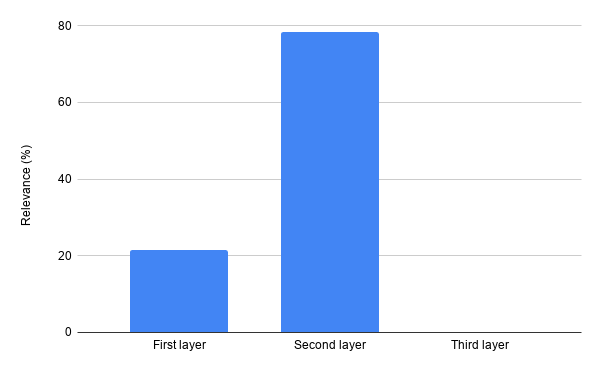
\includegraphics[width=\textwidth,height=8cm,keepaspectratio=true]
    {elmo-layers-relevance.png}
    \caption{
        Importance of ELMo layers in Constituent parsing
    }
    \label{fig:elmo-layers-relevance}
\end{figure}

\subsection{Primitive Tree analysis}

The model that gave best F1 score (95.87\%) is taken and their predicted syntax trees are compared against golden trees. All the noun and verb labels in the golden test dataset are compared against predicted labels and the accuracy is listed below:

\begin{figure}[H]
    \centering
    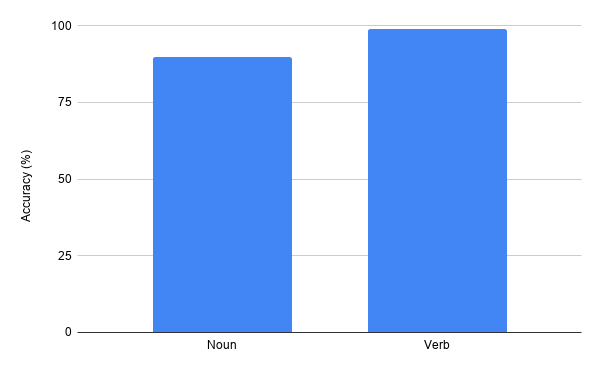
\includegraphics[width=\textwidth,height=8cm,keepaspectratio=true]
    {noun-verb-accuracy.png}
    \caption{
        Noun and Verb prediction accuracy 
    }
    \label{fig:noun-verb-accuracy}
\end{figure}

The model achieved an accuracy of 89.8\% and 99.0\% for noun and verb labels respectively. 

%\subsubsection{Distance analysis - meaning}
%Select the same words and see how the distance is. 

%\subsubsection{Tree analysis - what it captures and what it does not ?}


\pagebreak
\section{Conclusion and Future work}
% ----------------------------------------------------------------------------
During this thesis work, considerable attempts are put to build a constituent parser using neural networks. Over the past, Recurrent neural networks have been used in building a parser and also many NLP applications. In this, self-attention neural network modules are used intensively to understand sentences effectively. This understanding is used by a CKY decoder to predict the syntactic structure in a sentence. 

With multi-layered self-attention networks, constituent parsing achieves 93.68\% F1 score. Each of the self-attention heads learns distinct features and the heads in the higher layer learn abstract patterns. This is improved by using character and word embeddings as a representation of input. An F1 score of 94.10\% was the best achieved by constituent parser using only the dataset provided. 

With the help of external datasets such as German Wikipedia, pre-trained ELMo models are used as representative of input. The second layer of ELMo model has the greatest influence and combining all the layers with a weighted average achieves 95.87\% F1 score. So a self-attention module with ELMo based vectors as input representative achieves the maximum performance in building a constituent parser. 

The research work did not scope in the analysis of results along the lines of computational linguistics. With the help of experts, linguistic analysis has to be carried out which will give clarity on what parts of grammar identification needs to be improved. This information will help in building some of the hypotheses on how to improve and experiments can be carried out. It will also give an understanding of what self-attention module is good or bad at capturing.

Devlin et al. made efforts to build Bidirectional Encoder Representations from Transformers (BERT) \parencite{devlin2018bert} models which are the state of art techniques to represent text. This work achieved the best results for 11 NLP tasks such as MultiNLI with 86.7\%, and SQuAD v1.1 to 93.2\% F1 score. Pre-existing BERT based representations can be used for the input used in constituent parsing and see whether performance is improved or not.
% ----------------------------------------------------------------------------

% ----------------------------------------------------------------------------
\newpage
\printbibliography
\end{document}